\documentclass[aspectratio=169,11pt]{beamer}
\usepackage[T1]{fontenc}
\usepackage{lmodern}
\usepackage{graphicx}
\usepackage{xcolor}
\usepackage{tikz}
\usetikzlibrary{calc,positioning,arrows.meta}
\graphicspath{{figs/}}
\usefonttheme{professionalfonts}
\setbeamertemplate{navigation symbols}{}
\definecolor{owpaper}{HTML}{FBFAF6}
\definecolor{owink}{HTML}{16242E}
\definecolor{owdeep}{HTML}{0B2E4F}
\definecolor{owblue}{HTML}{1E6FB0}
\definecolor{owteal}{HTML}{0F8C8C}
\definecolor{owochre}{HTML}{D98A2B}
\definecolor{owmuted}{HTML}{5B6B78}
\setbeamercolor{background canvas}{bg=owpaper}
\setbeamercolor{normal text}{fg=owink}
\setbeamercolor{frametitle}{fg=owdeep}
\setbeamercolor{itemize item}{fg=owteal}
\setbeamercolor{itemize subitem}{fg=owochre}
\setbeamercolor{structure}{fg=owblue}
\setbeamerfont{frametitle}{series=\bfseries,size=\Large}
\setbeamertemplate{itemize item}{\small\raise0.5pt\hbox{\textbullet}}
\setbeamertemplate{frametitle}{%
  \vskip6pt\hbox{\color{owochre}\rule[2pt]{16pt}{2.2pt}}\hskip4pt
  \insertframetitle\par\vskip-2pt}
% nested-worlds mark
\newcommand{\owmark}[1][0.5]{\begin{tikzpicture}[scale=#1]
  \draw[owdeep,line width=1.1pt,rounded corners=1pt] (0,0) rectangle (1,1);
  \draw[owblue,line width=1.1pt,rounded corners=1pt] (0.22,0.22) rectangle (0.78,0.78);
  \fill[owteal,rounded corners=0.5pt] (0.40,0.40) rectangle (0.60,0.60);
\end{tikzpicture}}
\setbeamertemplate{footline}{\hbox{}\hfill{\color{owmuted}\tiny\insertframenumber}\hskip8pt\vskip4pt}

\begin{document}
\begin{frame}[plain]
\centering\vfill
{\owmark[1.4]}\par\vskip14pt
{\color{owdeep}\bfseries\LARGE Solving ARC-AGI-3 with Code World Models\par}\vskip8pt
{\color{owblue}\large First time all 25 games were solved without ever reading the game's code: the agent writes a little program that copies the game's rules, then figures out how to win\par}\vskip18pt
{\color{owink}\normalsize Jim Schwoebel --- Quome / OpenWorld\par}\vskip3pt
{\color{owmuted}\small github.com/quome-cloud/openworld\par}\vskip12pt

\includegraphics[width=1.7cm]{qr_openworld.png}\par\vskip2pt
{\color{owmuted}\scriptsize scan to open \& star the repo\par}
\vfill
\end{frame}

\begin{frame}{The whole talk on one map}\vfill\centering \resizebox{0.95\textwidth}{!}{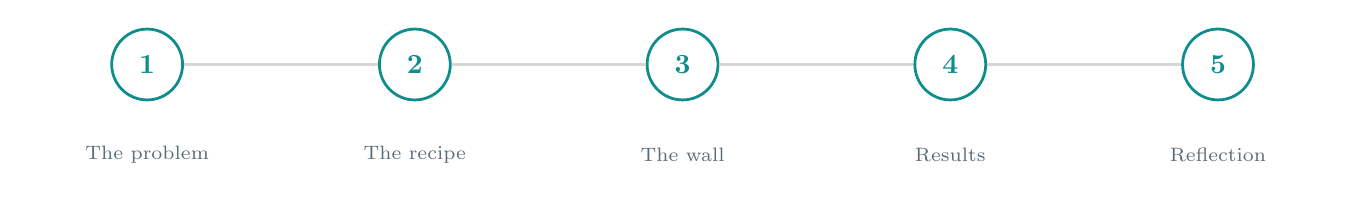
\begin{tikzpicture}[stn/.style={circle,draw=owteal,line width=1pt,minimum size=9mm,font=\bfseries,inner sep=0,text=owteal},std/.style={circle,draw=owteal,fill=owteal,line width=1pt,minimum size=9mm,font=\bfseries,inner sep=0,text=white},stc/.style={circle,draw=owochre,fill=owochre,line width=1.2pt,minimum size=11.5mm,font=\bfseries,inner sep=0,text=white},stx/.style={circle,draw=owmuted,line width=1pt,minimum size=9mm,font=\bfseries,inner sep=0,text=owmuted},stlbl/.style={font=\scriptsize,text=owmuted,align=center,text width=28mm},stln/.style={draw=black!16,line width=1.4pt}]\node[stn] (s0) at (0.0,0) {1};\node[stn] (s1) at (3.4,0) {2};\node[stn] (s2) at (6.8,0) {3};\node[stn] (s3) at (10.2,0) {4};\node[stn] (s4) at (13.6,0) {5};\node[stlbl] at (0.0,-1.15) {The problem};\node[stlbl] at (3.4,-1.15) {The recipe};\node[stlbl] at (6.8,-1.15) {The wall};\node[stlbl] at (10.2,-1.15) {Results};\node[stlbl] at (13.6,-1.15) {Reflection};\draw[stln] (s0)--(s1);\draw[stln] (s1)--(s2);\draw[stln] (s2)--(s3);\draw[stln] (s3)--(s4);\end{tikzpicture}}\vfill\end{frame}
\begin{frame}[plain]\vfill\centering \resizebox{0.95\textwidth}{!}{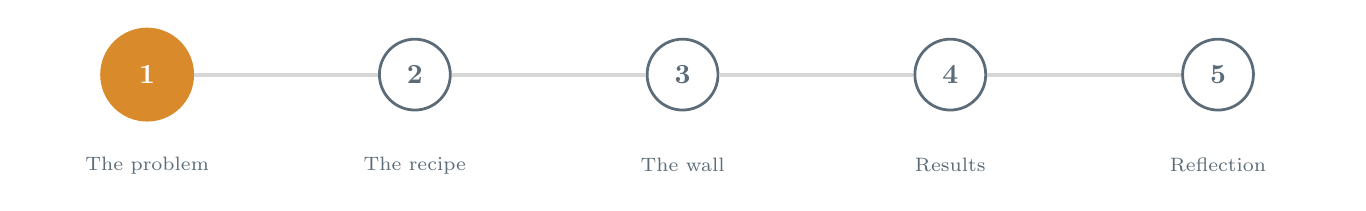
\begin{tikzpicture}[stn/.style={circle,draw=owteal,line width=1pt,minimum size=9mm,font=\bfseries,inner sep=0,text=owteal},std/.style={circle,draw=owteal,fill=owteal,line width=1pt,minimum size=9mm,font=\bfseries,inner sep=0,text=white},stc/.style={circle,draw=owochre,fill=owochre,line width=1.2pt,minimum size=11.5mm,font=\bfseries,inner sep=0,text=white},stx/.style={circle,draw=owmuted,line width=1pt,minimum size=9mm,font=\bfseries,inner sep=0,text=owmuted},stlbl/.style={font=\scriptsize,text=owmuted,align=center,text width=28mm},stln/.style={draw=black!16,line width=1.4pt}]\node[stc] (s0) at (0.0,0) {1};\node[stx] (s1) at (3.4,0) {2};\node[stx] (s2) at (6.8,0) {3};\node[stx] (s3) at (10.2,0) {4};\node[stx] (s4) at (13.6,0) {5};\node[stlbl] at (0.0,-1.15) {The problem};\node[stlbl] at (3.4,-1.15) {The recipe};\node[stlbl] at (6.8,-1.15) {The wall};\node[stlbl] at (10.2,-1.15) {Results};\node[stlbl] at (13.6,-1.15) {Reflection};\draw[stln] (s0)--(s1);\draw[stln] (s1)--(s2);\draw[stln] (s2)--(s3);\draw[stln] (s3)--(s4);\end{tikzpicture}}\\[24pt]
{\color{owochre}\bfseries\footnotesize PART 1}\\[5pt]
{\color{owdeep}\bfseries\Large The problem}\\[10pt]{\color{owmuted}\large What ARC-AGI-3 is, and why it is hard}\vfill\end{frame}
\begin{frame}{Puzzles you can only crack by playing}\vfill
\begin{columns}[T]
\begin{column}{0.46\textwidth}{\color{owmuted}\bfseries\large Old ARC}\par\medskip\begin{itemize}\small \item Look at a before-and-after grid
\item Spot the pattern\end{itemize}\end{column}
\begin{column}{0.46\textwidth}{\color{owteal}\bfseries\large ARC-AGI-3}\par\medskip\begin{itemize}\small \item Little video-game puzzles: learn the rules and the goal only by playing
\item A 64x64 grid of dots, 16 colors, 6 to 10 levels
\item Screen only: no words, no outside knowledge
\item Tests exploring, learning how things move, guessing the goal, and planning\end{itemize}\end{column}
\end{columns}\vfill\end{frame}
\begin{frame}{A real example: the game ka59}
\centering
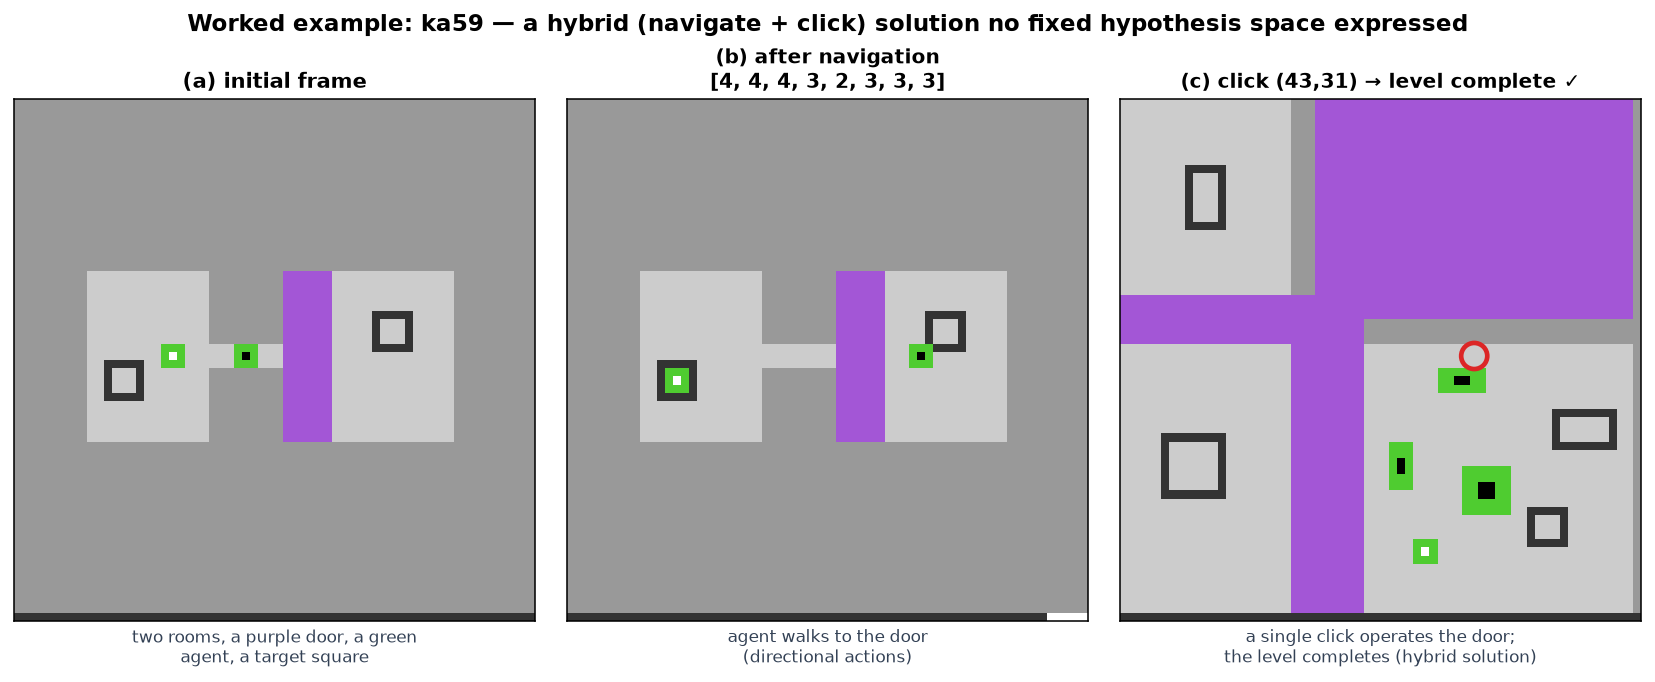
\includegraphics[width=\linewidth,height=0.48\textheight,keepaspectratio]{arc3_example_ka59.png}\vskip3pt{\color{owmuted}\footnotesize Two rooms, a hallway, a purple door: walk over, then click to clear the level\par}
\flushleft \vskip3pt{\footnotesize \begin{itemize}
  \item The agent is told nothing: no rules, no goal in words
  \item You can move (buttons 1-5,7) or click a spot on the grid (ACTION6)
  \item Winning is a set of steps in the right order, not one good screen
\end{itemize}}
\end{frame}
\begin{frame}{Why it is hard}\vfill\begin{center}{\color{owteal}\fontsize{58}{62}\selectfont\bfseries <1\%}\par\vskip10pt{\color{owdeep}\large best AI scored, March 2026}\end{center}\vskip10pt\begin{itemize}\item People solve every one of these games -- 100\%\item No instructions: you discover how to win on your own\item A win takes many steps, and you get nothing until the very end\end{itemize}\vfill\end{frame}
\begin{frame}[plain]\centering\vfill
{\color{owdeep}\bfseries\LARGE The hard part is not copying how the game works. It is figuring out what you are supposed to be doing.\par}\vfill\end{frame}
\begin{frame}[plain]\vfill\centering \resizebox{0.95\textwidth}{!}{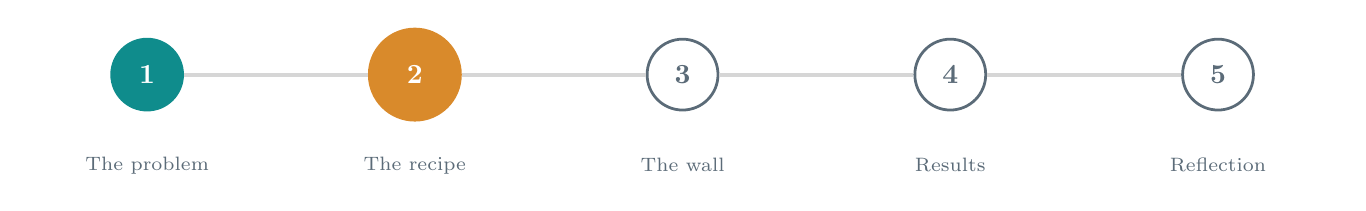
\begin{tikzpicture}[stn/.style={circle,draw=owteal,line width=1pt,minimum size=9mm,font=\bfseries,inner sep=0,text=owteal},std/.style={circle,draw=owteal,fill=owteal,line width=1pt,minimum size=9mm,font=\bfseries,inner sep=0,text=white},stc/.style={circle,draw=owochre,fill=owochre,line width=1.2pt,minimum size=11.5mm,font=\bfseries,inner sep=0,text=white},stx/.style={circle,draw=owmuted,line width=1pt,minimum size=9mm,font=\bfseries,inner sep=0,text=owmuted},stlbl/.style={font=\scriptsize,text=owmuted,align=center,text width=28mm},stln/.style={draw=black!16,line width=1.4pt}]\node[std] (s0) at (0.0,0) {1};\node[stc] (s1) at (3.4,0) {2};\node[stx] (s2) at (6.8,0) {3};\node[stx] (s3) at (10.2,0) {4};\node[stx] (s4) at (13.6,0) {5};\node[stlbl] at (0.0,-1.15) {The problem};\node[stlbl] at (3.4,-1.15) {The recipe};\node[stlbl] at (6.8,-1.15) {The wall};\node[stlbl] at (10.2,-1.15) {Results};\node[stlbl] at (13.6,-1.15) {Reflection};\draw[stln] (s0)--(s1);\draw[stln] (s1)--(s2);\draw[stln] (s2)--(s3);\draw[stln] (s3)--(s4);\end{tikzpicture}}\\[24pt]
{\color{owochre}\bfseries\footnotesize PART 2}\\[5pt]
{\color{owdeep}\bfseries\Large The recipe}\\[10pt]{\color{owmuted}\large Write a rule-copy program by playing, and keep checking it}\vfill\end{frame}
\begin{frame}{The loop, in six steps}\vfill\centering
\resizebox{0.98\textwidth}{!}{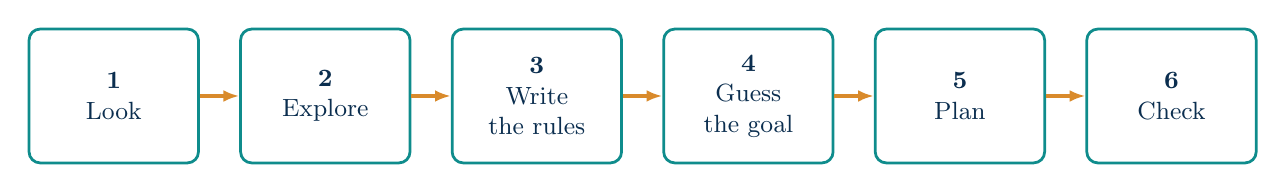
\begin{tikzpicture}[node distance=5mm and 5mm,
  sb/.style={draw=owteal,line width=1pt,rounded corners=4pt,fill=white,inner sep=5pt,
  text width=18mm,align=center,minimum height=17mm,font=\small,text=owdeep}]
\node[sb] (n0) {\textbf{1}\\ Look};\node[sb,right=of n0] (n1) {\textbf{2}\\ Explore};\node[sb,right=of n1] (n2) {\textbf{3}\\ Write the rules};\node[sb,right=of n2] (n3) {\textbf{4}\\ Guess the goal};\node[sb,right=of n3] (n4) {\textbf{5}\\ Plan};\node[sb,right=of n4] (n5) {\textbf{6}\\ Check};
\draw[-{Latex[length=2mm]},owochre,line width=1.1pt] (n0) -- (n1);\draw[-{Latex[length=2mm]},owochre,line width=1.1pt] (n1) -- (n2);\draw[-{Latex[length=2mm]},owochre,line width=1.1pt] (n2) -- (n3);\draw[-{Latex[length=2mm]},owochre,line width=1.1pt] (n3) -- (n4);\draw[-{Latex[length=2mm]},owochre,line width=1.1pt] (n4) -- (n5);
\end{tikzpicture}}\vfill\end{frame}
\begin{frame}{How the agent solves a game}
\centering
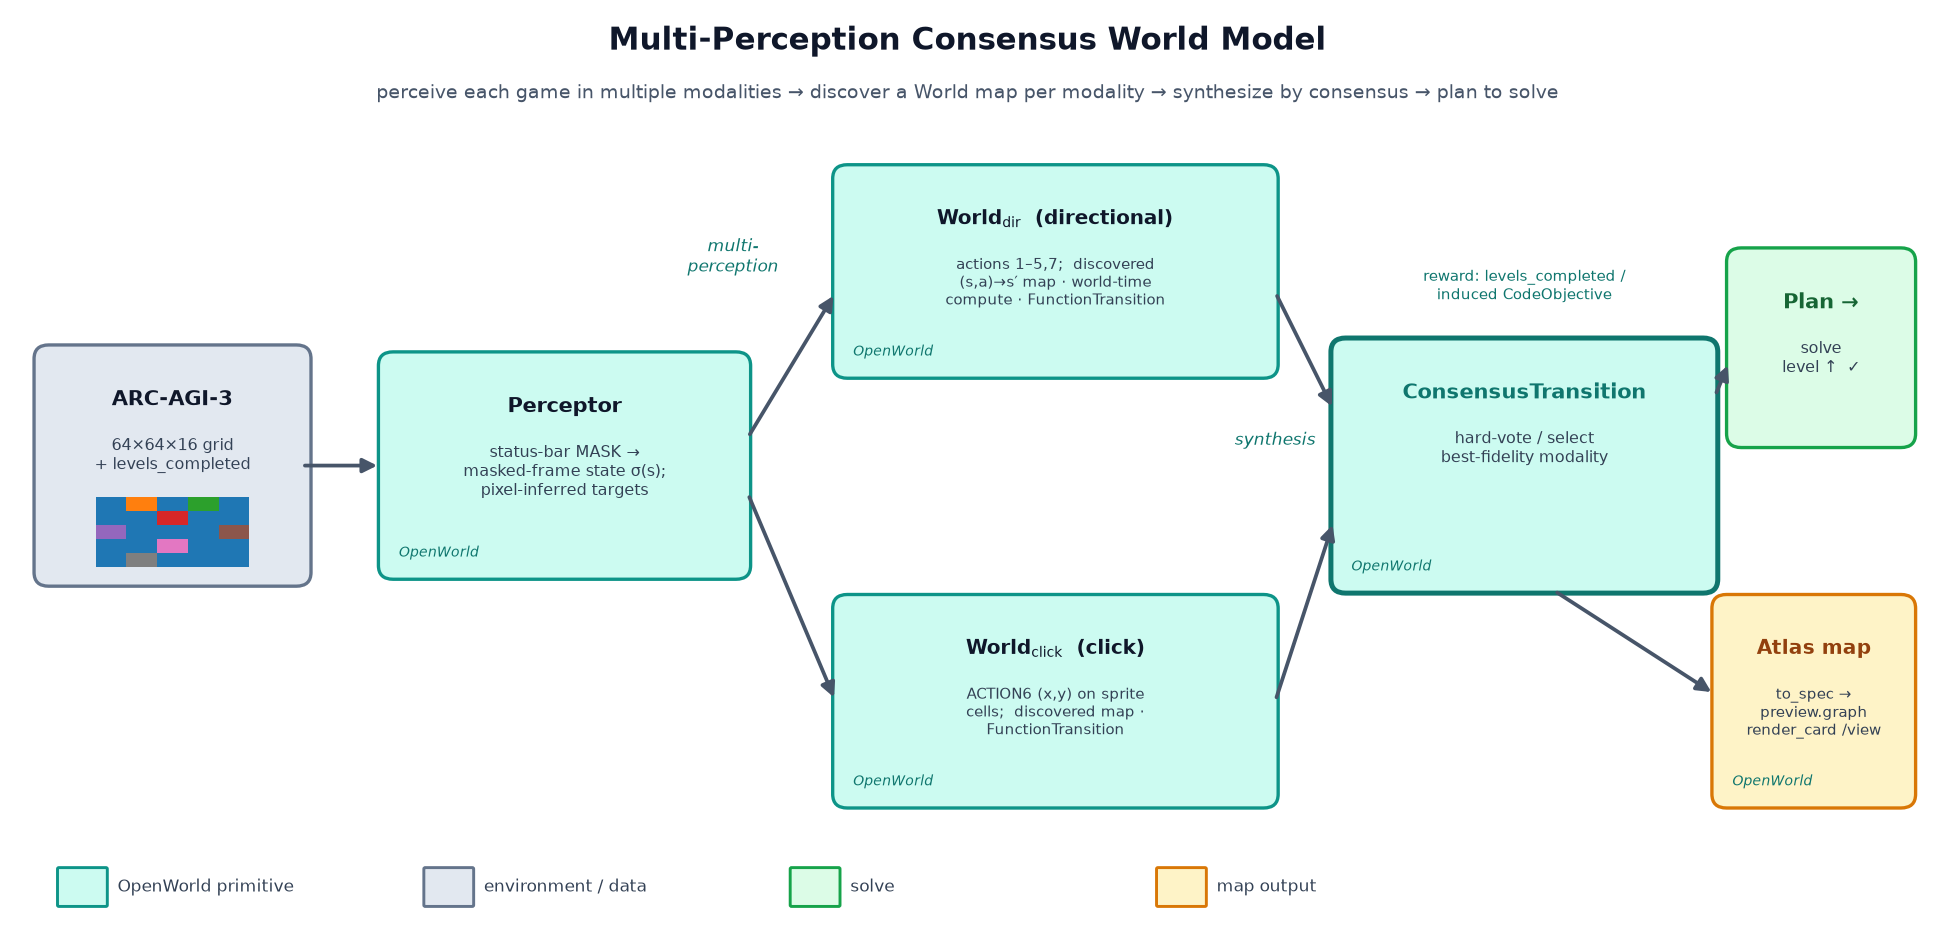
\includegraphics[width=\linewidth,height=0.48\textheight,keepaspectratio]{arc3_architecture.png}\vskip3pt{\color{owmuted}\footnotesize Look -> explore -> write the rules as code -> guess the goal -> plan -> re-play the moves to prove it works\par}
\flushleft \vskip3pt{\footnotesize \begin{itemize}
  \item Kept in a locked box that never reads the game's code
  \item Turns the picture into simple facts about what is on the screen
  \item Every solve becomes a working world you can open and play
\end{itemize}}
\end{frame}
\begin{frame}{The loop, in plain words}\vfill\begin{enumerate}\item \textbf{Poke around} --- Act, and note 'from this screen, this button gave that screen'\item \textbf{Write the rule} --- A little program predicts the next screen; keep it only if unseen examples come out exactly right (check 1)\item \textbf{Guess the goal} --- What makes the level counter go up?\item \textbf{Plan and prove} --- Plan inside the program, then re-play the moves against the real game (check 2)\end{enumerate}\vfill\end{frame}
\begin{frame}{What a world model is made of}
\centering
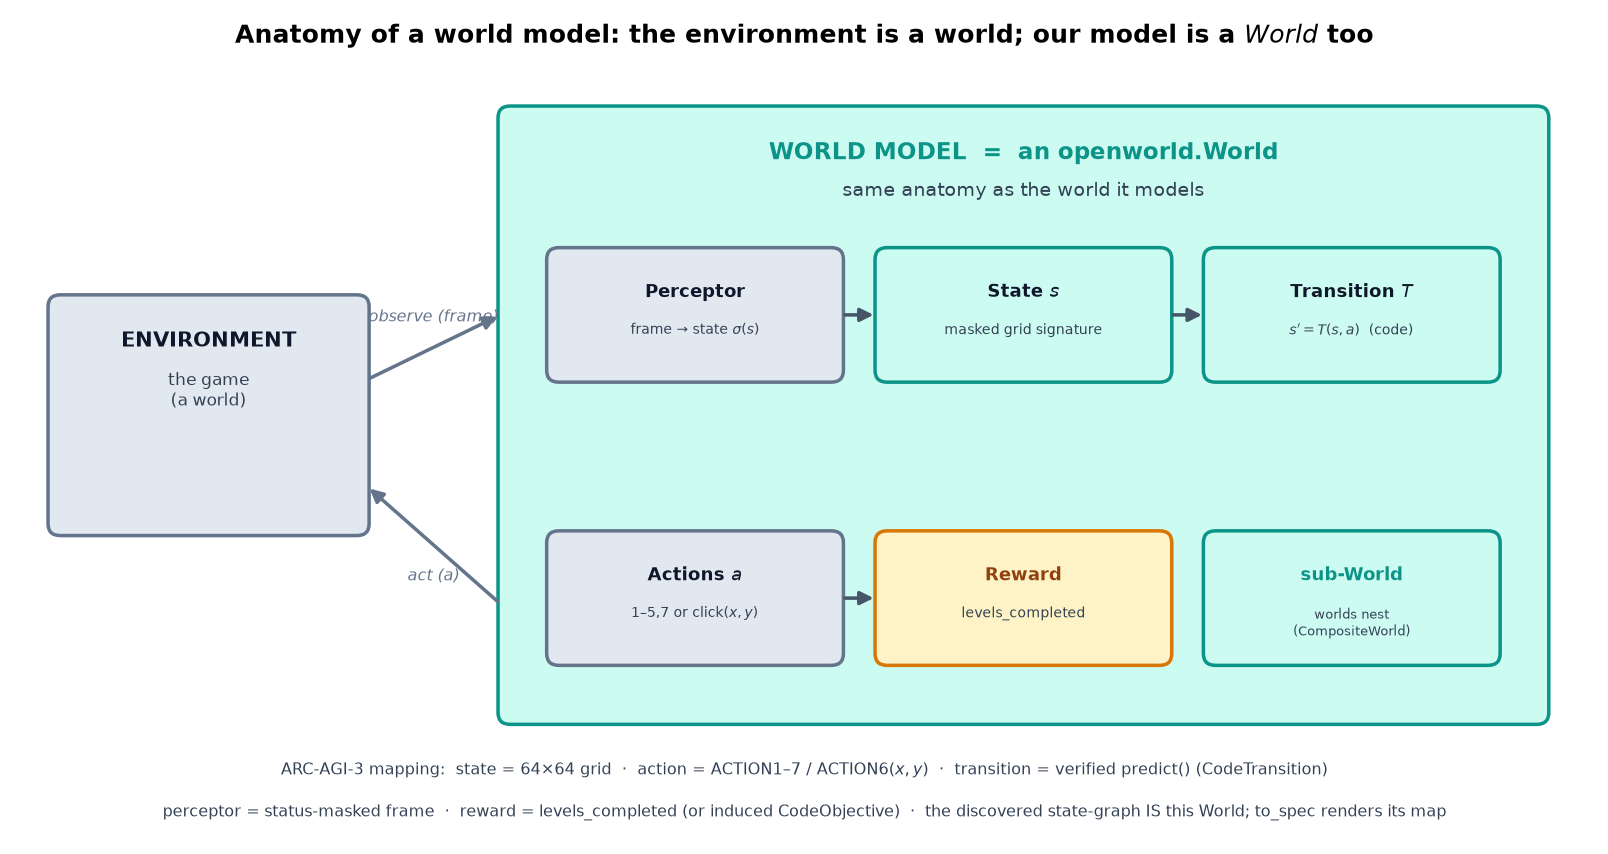
\includegraphics[width=\linewidth,height=0.48\textheight,keepaspectratio]{arc3_anatomy.png}\vskip3pt{\color{owmuted}\footnotesize The copy of a game is itself a little world -- same five parts, and worlds fit inside worlds\par}
\flushleft \vskip3pt{\footnotesize \begin{itemize}
  \item Where things are, what you can do, how it changes, what you see, what counts as good
  \item Copying a game means building a world whose changes match the real one
  \item A world can hold another world inside it
\end{itemize}}
\end{frame}
\begin{frame}[plain]\centering\vfill
{\color{owochre}\rule{40pt}{2.5pt}}\par\vskip10pt
{\color{owdeep}\bfseries\Large Copying the game is not the wall\par}\vfill\end{frame}
\begin{frame}{The copy of the game is just code}\vfill\begin{columns}[T]\begin{column}{.46\textwidth}{\color{owdeep}\bfseries Repeatable}\\[2pt]{\color{owmuted}\small Same move, same result, every time (score 1.00)}\end{column}\begin{column}{.46\textwidth}{\color{owdeep}\bfseries Written as code}\\[2pt]{\color{owmuted}\small So the rules can be written out exactly, as Python}\end{column}\end{columns}\vskip12pt\begin{columns}[T]\begin{column}{.46\textwidth}{\color{owdeep}\bfseries Only if passes}\\[2pt]{\color{owmuted}\small A program is kept only if it gets unseen examples exactly right}\end{column}\begin{column}{.46\textwidth}{\color{owdeep}\bfseries Claude 49\%}\\[2pt]{\color{owmuted}\small On 21 changing games, got the whole next screen right 49\% of the time; 3 nearly perfect, small local models almost nothing}\end{column}\end{columns}\vfill\end{frame}
\begin{frame}{How well each model copies the rules}
\centering

\includegraphics[width=\linewidth,height=0.48\textheight,keepaspectratio]{arc3_fidelity.png}\vskip3pt{\color{owmuted}\footnotesize Claude rewrites the game's rules as working code far better than the small local models\par}
\flushleft \vskip3pt{\footnotesize \begin{itemize}
  \item One wrong dot in the 64x64 screen and it fails the check
  \item The smarter model wins big: qwen-32B and qwen-7B are far behind
  \item This only tests next-screen accuracy -- no games are won here, on purpose
\end{itemize}}
\end{frame}
\begin{frame}[plain]\centering\vfill
{\color{owdeep}\bfseries\LARGE The rules can be copied exactly, as checked code. Building the copy of the game is the easy half.\par}\vfill\end{frame}
\begin{frame}[plain]\vfill\centering \resizebox{0.95\textwidth}{!}{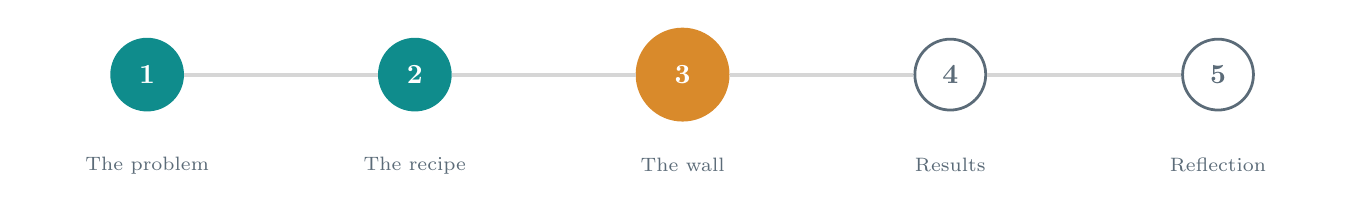
\begin{tikzpicture}[stn/.style={circle,draw=owteal,line width=1pt,minimum size=9mm,font=\bfseries,inner sep=0,text=owteal},std/.style={circle,draw=owteal,fill=owteal,line width=1pt,minimum size=9mm,font=\bfseries,inner sep=0,text=white},stc/.style={circle,draw=owochre,fill=owochre,line width=1.2pt,minimum size=11.5mm,font=\bfseries,inner sep=0,text=white},stx/.style={circle,draw=owmuted,line width=1pt,minimum size=9mm,font=\bfseries,inner sep=0,text=owmuted},stlbl/.style={font=\scriptsize,text=owmuted,align=center,text width=28mm},stln/.style={draw=black!16,line width=1.4pt}]\node[std] (s0) at (0.0,0) {1};\node[std] (s1) at (3.4,0) {2};\node[stc] (s2) at (6.8,0) {3};\node[stx] (s3) at (10.2,0) {4};\node[stx] (s4) at (13.6,0) {5};\node[stlbl] at (0.0,-1.15) {The problem};\node[stlbl] at (3.4,-1.15) {The recipe};\node[stlbl] at (6.8,-1.15) {The wall};\node[stlbl] at (10.2,-1.15) {Results};\node[stlbl] at (13.6,-1.15) {Reflection};\draw[stln] (s0)--(s1);\draw[stln] (s1)--(s2);\draw[stln] (s2)--(s3);\draw[stln] (s3)--(s4);\end{tikzpicture}}\\[24pt]
{\color{owochre}\bfseries\footnotesize PART 3}\\[5pt]
{\color{owdeep}\bfseries\Large The wall}\\[10pt]{\color{owmuted}\large A win is a recipe of steps in order, not one good screen}\vfill\end{frame}
\begin{frame}{One good screen vs a recipe of steps}\centering
\includegraphics[width=\linewidth,height=0.74\textheight,keepaspectratio]{arc3_goal_as_procedure.png}\end{frame}
\begin{frame}{Four careful ways to guess the goal -- all fail (0), even with a perfect copy of the rules}\vfill\begin{columns}[T]\begin{column}{.46\textwidth}{\color{owdeep}\bfseries Simple goals}\\[2pt]{\color{owmuted}\small Get here / cover this / collect that: 0}\end{column}\begin{column}{.46\textwidth}{\color{owdeep}\bfseries Ask top AI}\\[2pt]{\color{owmuted}\small Guess the goal, with and without feedback: 0}\end{column}\end{columns}\vskip12pt\begin{columns}[T]\begin{column}{.46\textwidth}{\color{owdeep}\bfseries Nested worlds}\\[2pt]{\color{owmuted}\small Reason about goals across the sub-worlds: 0}\end{column}\begin{column}{.46\textwidth}{\color{owdeep}\bfseries Rebuild engine}\\[2pt]{\color{owmuted}\small Rebuild from play and prove a goal: 0}\end{column}\end{columns}\vfill\end{frame}
\begin{frame}{Why guessing the goal by machine cannot cross it}\vfill\begin{itemize}\item \textbf{Tiny corner} --- Exploring touches only 50-138 screens and never trips the reward\item \textbf{One-shot} --- On s5i5 it thinks a timer is the goal\item \textbf{Thin feedback} --- It only says 'wrong', never 'warmer'; a huge cold brute-force sweep (E146) won 0 new games\item \textbf{The wall} --- The stuck point is guessing the goal -- not copying, planning, or exploring\end{itemize}\vfill\end{frame}
\begin{frame}[plain]\centering\vfill
{\color{owdeep}\bfseries\LARGE A copy of the game is useless until it holds a proven path to the win. Exploring more of the game does not help.\par}\vfill\end{frame}
\begin{frame}[plain]\centering\vfill
{\color{owochre}\rule{40pt}{2.5pt}}\par\vskip10pt
{\color{owdeep}\bfseries\Large The landscape of approaches\par}\vfill\end{frame}
\begin{frame}{Which approach solves which game}
\centering

\includegraphics[width=\linewidth,height=0.48\textheight,keepaspectratio]{arc3_strategy_heatmap.png}\vskip3pt{\color{owmuted}\footnotesize The goal-guessing columns are empty; only the reasoning agent lights up the hard games\par}
\flushleft \vskip3pt{\footnotesize \begin{itemize}
  \item Directed search and map-building each solve 6 games
  \item Combining several ways of seeing reaches 10 (best of the automatic tiers)
  \item The live coding agent lights up the recipe-walls nothing else can touch
\end{itemize}}
\end{frame}
\begin{frame}{Three kinds of approach}\vfill
\begin{columns}[T]
\begin{column}{0.46\textwidth}{\color{owmuted}\bfseries\large Automatic ways}\par\medskip\begin{itemize}\small \item Guess the goal: all fail -- 0 hard games, even with a perfect copy
\item Seeing and searching: only games you can stumble into\end{itemize}\end{column}
\begin{column}{0.46\textwidth}{\color{owteal}\bfseries\large Reasoning agent}\par\medskip\begin{itemize}\small \item The only way that crosses the walls\end{itemize}\end{column}
\end{columns}\vfill\end{frame}
\begin{frame}{The reasoning agent that writes its own copy of the game}\vfill\begin{center}{\color{owteal}\fontsize{58}{62}\selectfont\bfseries 15 of 25}\par\vskip10pt{\color{owdeep}\large the live agent, on its own}\end{center}\vskip10pt\begin{itemize}\item Claude Code: one working session per game, no trying over and over\item The prompt gives only the controls and the recipe -- never how to win\item Crosses every wall the automatic ways miss (dc22, g50t, ka59, ...)\item Reasons out the goal instead of searching a fixed list of guesses\end{itemize}\vfill\end{frame}
\begin{frame}[plain]\vfill\centering \resizebox{0.95\textwidth}{!}{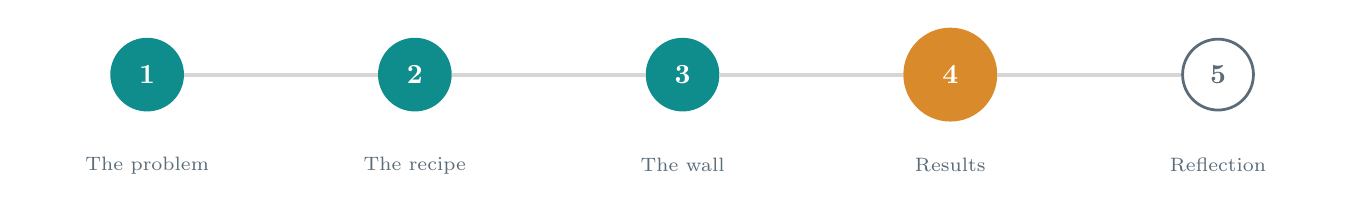
\begin{tikzpicture}[stn/.style={circle,draw=owteal,line width=1pt,minimum size=9mm,font=\bfseries,inner sep=0,text=owteal},std/.style={circle,draw=owteal,fill=owteal,line width=1pt,minimum size=9mm,font=\bfseries,inner sep=0,text=white},stc/.style={circle,draw=owochre,fill=owochre,line width=1.2pt,minimum size=11.5mm,font=\bfseries,inner sep=0,text=white},stx/.style={circle,draw=owmuted,line width=1pt,minimum size=9mm,font=\bfseries,inner sep=0,text=owmuted},stlbl/.style={font=\scriptsize,text=owmuted,align=center,text width=28mm},stln/.style={draw=black!16,line width=1.4pt}]\node[std] (s0) at (0.0,0) {1};\node[std] (s1) at (3.4,0) {2};\node[std] (s2) at (6.8,0) {3};\node[stc] (s3) at (10.2,0) {4};\node[stx] (s4) at (13.6,0) {5};\node[stlbl] at (0.0,-1.15) {The problem};\node[stlbl] at (3.4,-1.15) {The recipe};\node[stlbl] at (6.8,-1.15) {The wall};\node[stlbl] at (10.2,-1.15) {Results};\node[stlbl] at (13.6,-1.15) {Reflection};\draw[stln] (s0)--(s1);\draw[stln] (s1)--(s2);\draw[stln] (s2)--(s3);\draw[stln] (s3)--(s4);\end{tikzpicture}}\\[24pt]
{\color{owochre}\bfseries\footnotesize PART 4}\\[5pt]
{\color{owdeep}\bfseries\Large Results}\\[10pt]{\color{owmuted}\large All 25 solved, a stronger model solves more, and the atlas}\vfill\end{frame}
\begin{frame}{The first time every game was solved this way}\vfill\begin{columns}[c]\begin{column}{0.323\textwidth}\centering{\color{owochre}\fontsize{40}{44}\selectfont\bfseries 25/25}\\[6pt]{\color{owmuted}\small games, no code read}\end{column}\begin{column}{0.323\textwidth}\centering{\color{owdeep}\fontsize{40}{44}\selectfont\bfseries 183/183}\\[6pt]{\color{owmuted}\small levels solved}\end{column}\begin{column}{0.323\textwidth}\centering{\color{owdeep}\fontsize{40}{44}\selectfont\bfseries 1st}\\[6pt]{\color{owmuted}\small perfect run}\end{column}\end{columns}\vfill\end{frame}
\begin{frame}{Every game solved, one by one (a stronger model solves more)}
\centering
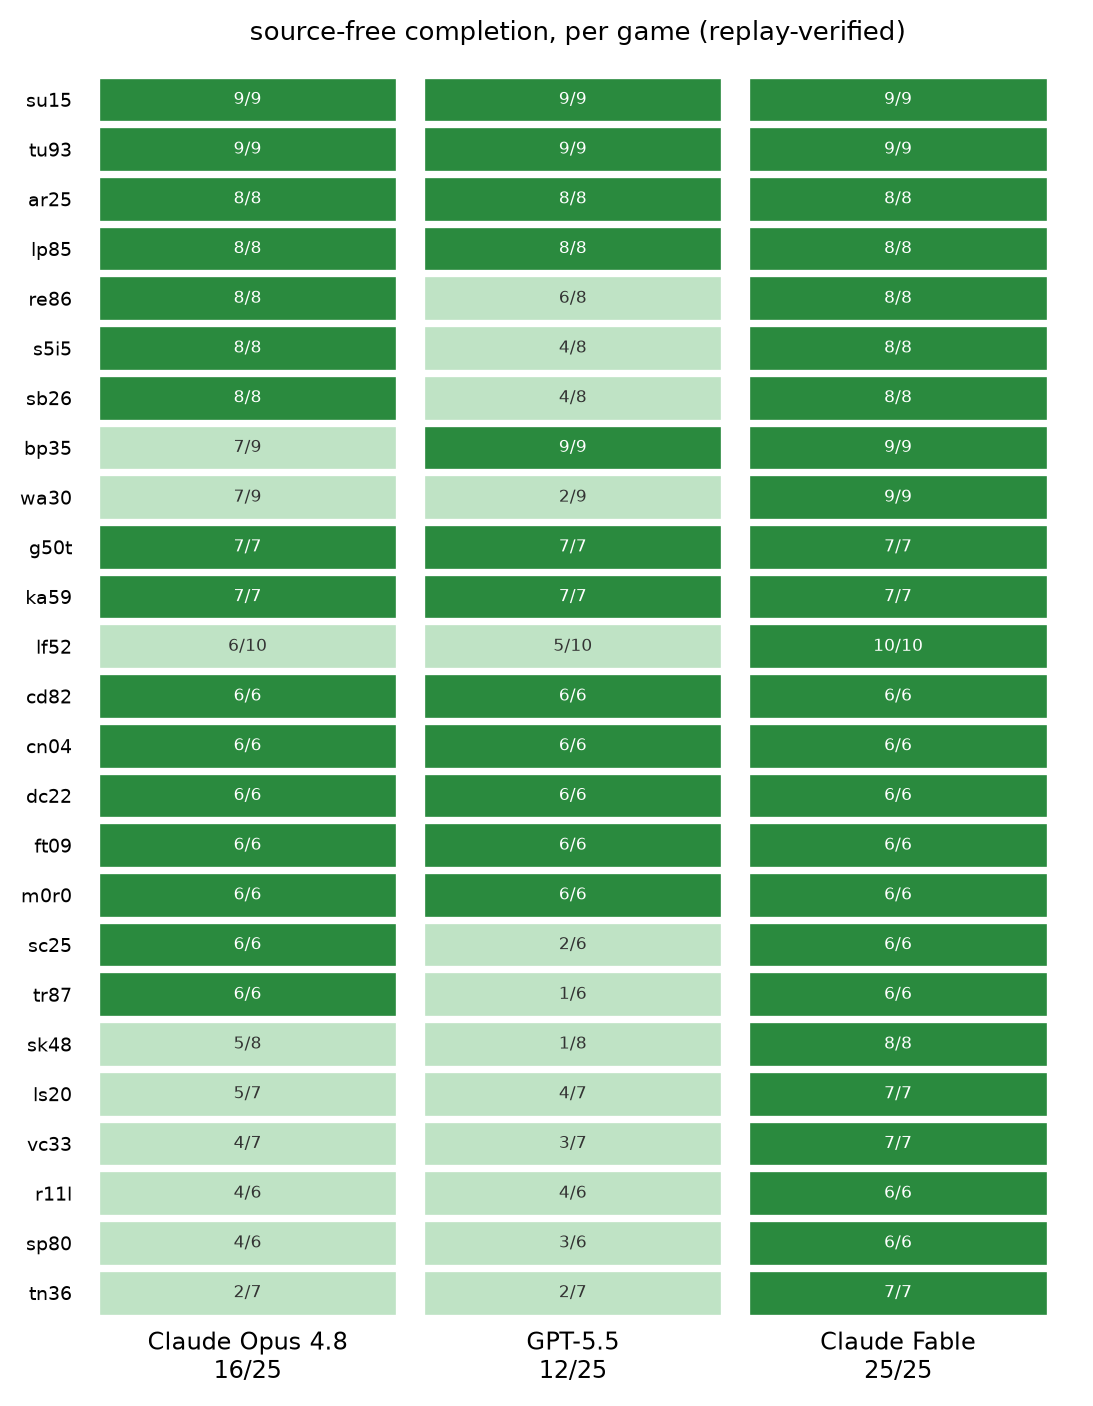
\includegraphics[width=\linewidth,height=0.48\textheight,keepaspectratio]{arc3_source_matrix.png}\vskip3pt{\color{owmuted}\footnotesize Claude Fable clears all 25 games; a stronger model clears more walls for the same budget\par}
\flushleft \vskip3pt{\footnotesize \begin{itemize}
  \item Claude Fable 5: 25/25 games, 183/183 levels -- the first perfect run
  \item Main run Claude Opus 4.8: 16/25 (158 levels) on the exact same setup
  \item GPT-5.5: 12/25; best earlier work (baseline1): 15/25 (145 levels)
  \item All proven by re-playing the moves; none use stored answers
\end{itemize}}
\end{frame}
\begin{frame}{The headline numbers, read carefully}\vfill\begin{itemize}\item \textbf{25/25} --- Fable with no code read, done 2026-07-04 09:05:14 UTC\item \textbf{Beats best} --- On games, levels, and how few moves it used\item \textbf{lf52} --- Clears the one level no earlier run ever solved\item \textbf{Runnable} --- Every solved game is a real world you can run and open; public games only, the private hidden set was untouched\end{itemize}\vfill\end{frame}
\begin{frame}{A stronger model clears more walls}
\centering
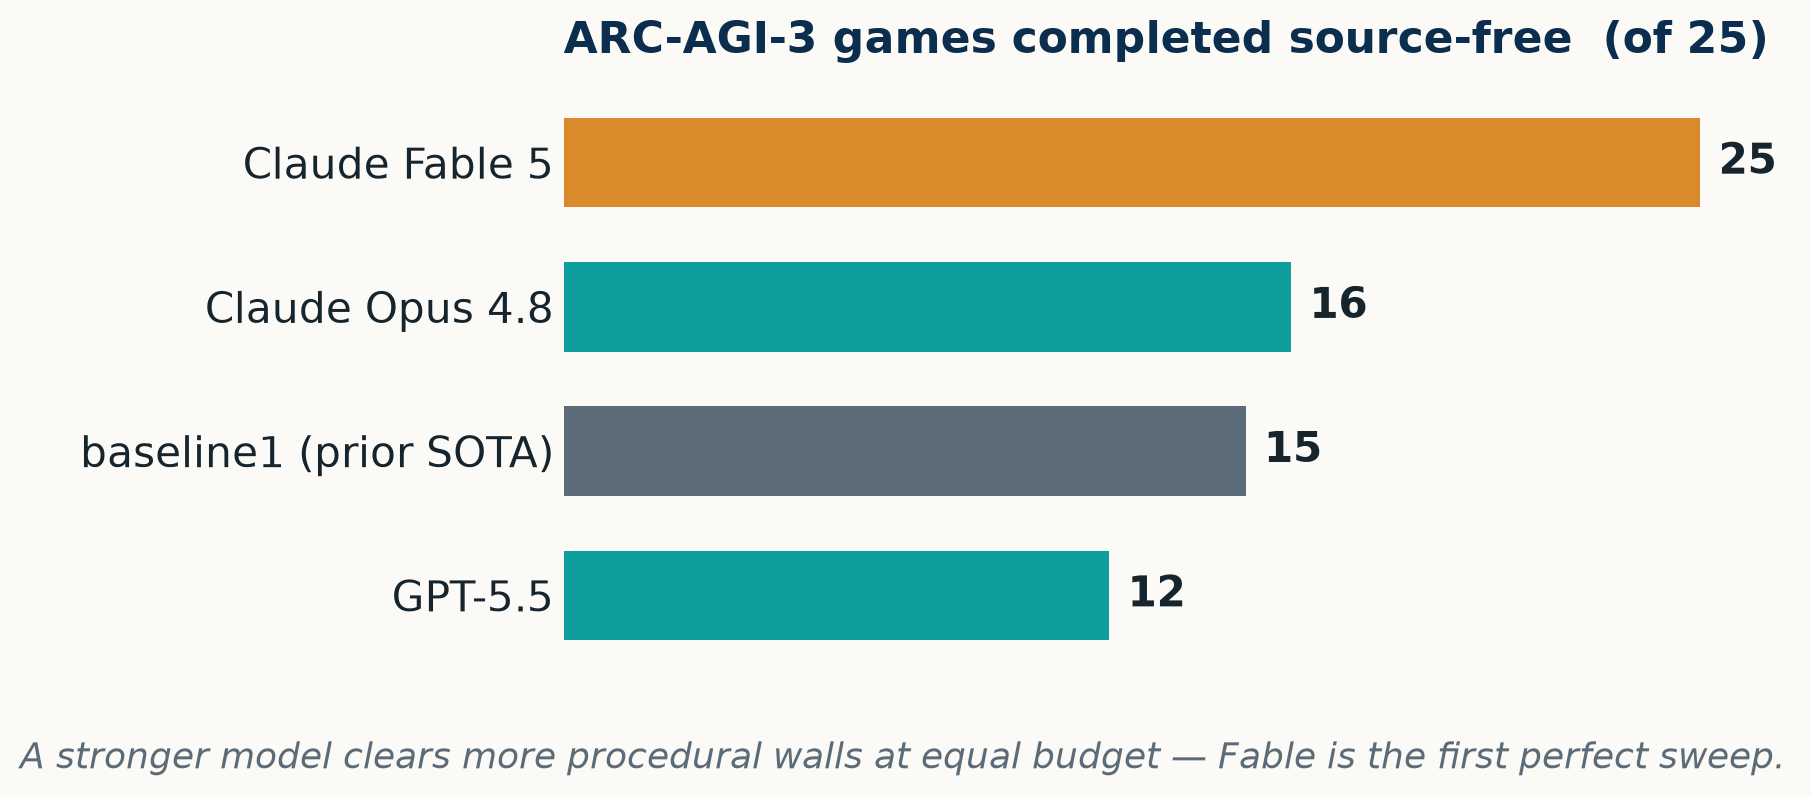
\includegraphics[width=\linewidth,height=0.48\textheight,keepaspectratio]{pres_arc3_scaling.png}\vskip3pt{\color{owmuted}\footnotesize Same setup, same prompt, same budget -- only the model changes\par}
\flushleft \vskip3pt{\footnotesize \begin{itemize}
  \item GPT-5.5 12 -> Opus 16 -> Fable 25 of 25 games
  \item Fable finds each solve using about 3.5x less text (23M vs 81M)
\end{itemize}}
\end{frame}
\begin{frame}{How few moves it used, per level (Fable, no code read)}
\centering
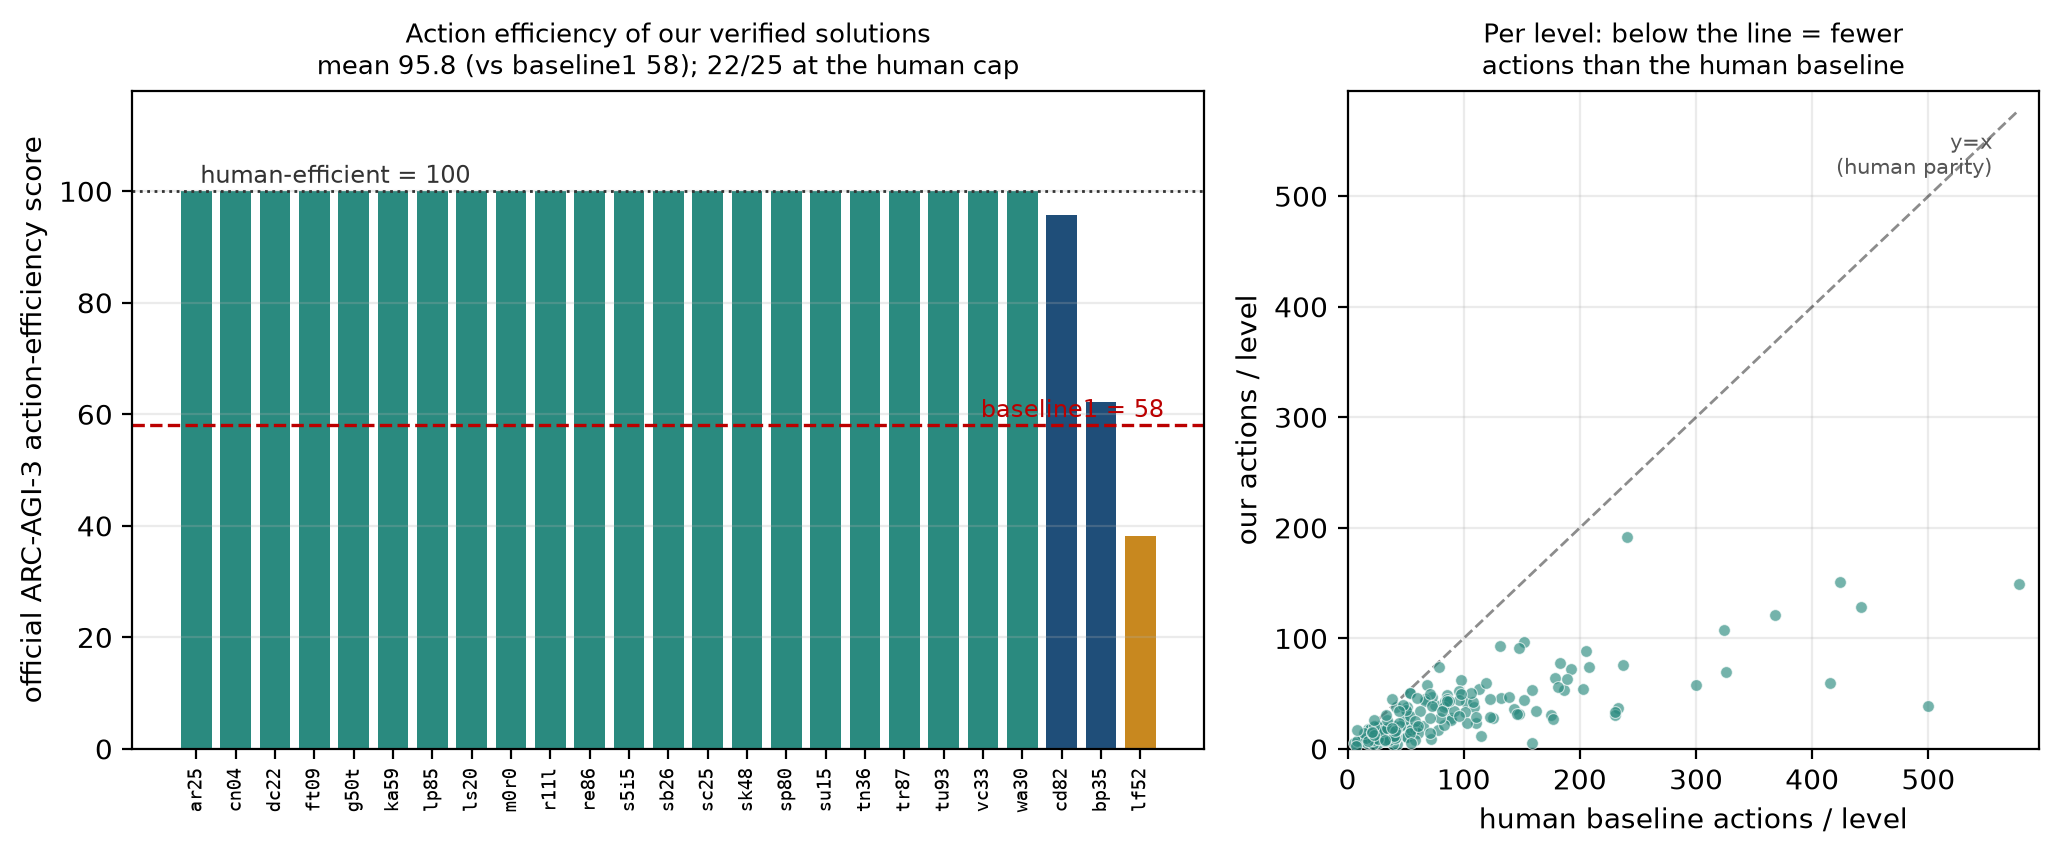
\includegraphics[width=\linewidth,height=0.48\textheight,keepaspectratio]{arc3_rhae.png}\vskip3pt{\color{owmuted}\footnotesize Every game matches or beats a person; per-level score min((b/a)\textasciicircum{}2 * 100, 115)\par}
\flushleft \vskip3pt{\footnotesize \begin{itemize}
  \item Fable used far fewer moves than a person: score 100.0 vs the earlier best's 58 (\textasciitilde{}72\% better)
  \item 174 of 183 levels beat the person; 168 hit the top score of 115
  \item Moves per level are usually about a third of a person's
  \item Scored by the game's own tool -- we did not rebuild the measure
\end{itemize}}
\end{frame}
\begin{frame}{An honest baseline: levels reached vs random play}
\centering

\includegraphics[width=\linewidth,height=0.48\textheight,keepaspectratio]{arc3_above_random.png}\vskip3pt{\color{owmuted}\footnotesize Random play reaches the first level of 11/25, but finishes 0 games all the way\par}
\flushleft \vskip3pt{\footnotesize \begin{itemize}
  \item With unlimited free restarts offline, about half the 'reached one level' count is free
  \item One 'solve' (lp85, one click over and over) is no better than random
  \item What really counts: 14 games random never even reaches (the walls)
  \item So we report 16/25 as clearly better than random
\end{itemize}}
\end{frame}
\begin{frame}[plain]\centering\vfill
{\color{owochre}\rule{40pt}{2.5pt}}\par\vskip10pt
{\color{owdeep}\bfseries\Large The atlas: every solve is a world\par}\vfill\end{frame}
\begin{frame}{25 games, 25 working worlds you can open}
\centering

\includegraphics[width=\linewidth,height=0.48\textheight,keepaspectratio]{arc3_maps_gallery.png}\vskip3pt{\color{owmuted}\footnotesize A winning screen from Fable's from-scratch solve of every game\par}
\flushleft \vskip3pt{\footnotesize \begin{itemize}
  \item Each solve: turn the picture into facts -> a rules program -> a goal check
  \item Saves as a one-page atlas card, and runs at openworld serve /view
  \item 25 clearly different worlds: moving, clicking, box-pushing, mirrors, building
\end{itemize}}
\end{frame}
\begin{frame}{Example solve: ka59 (7/7)}
\centering
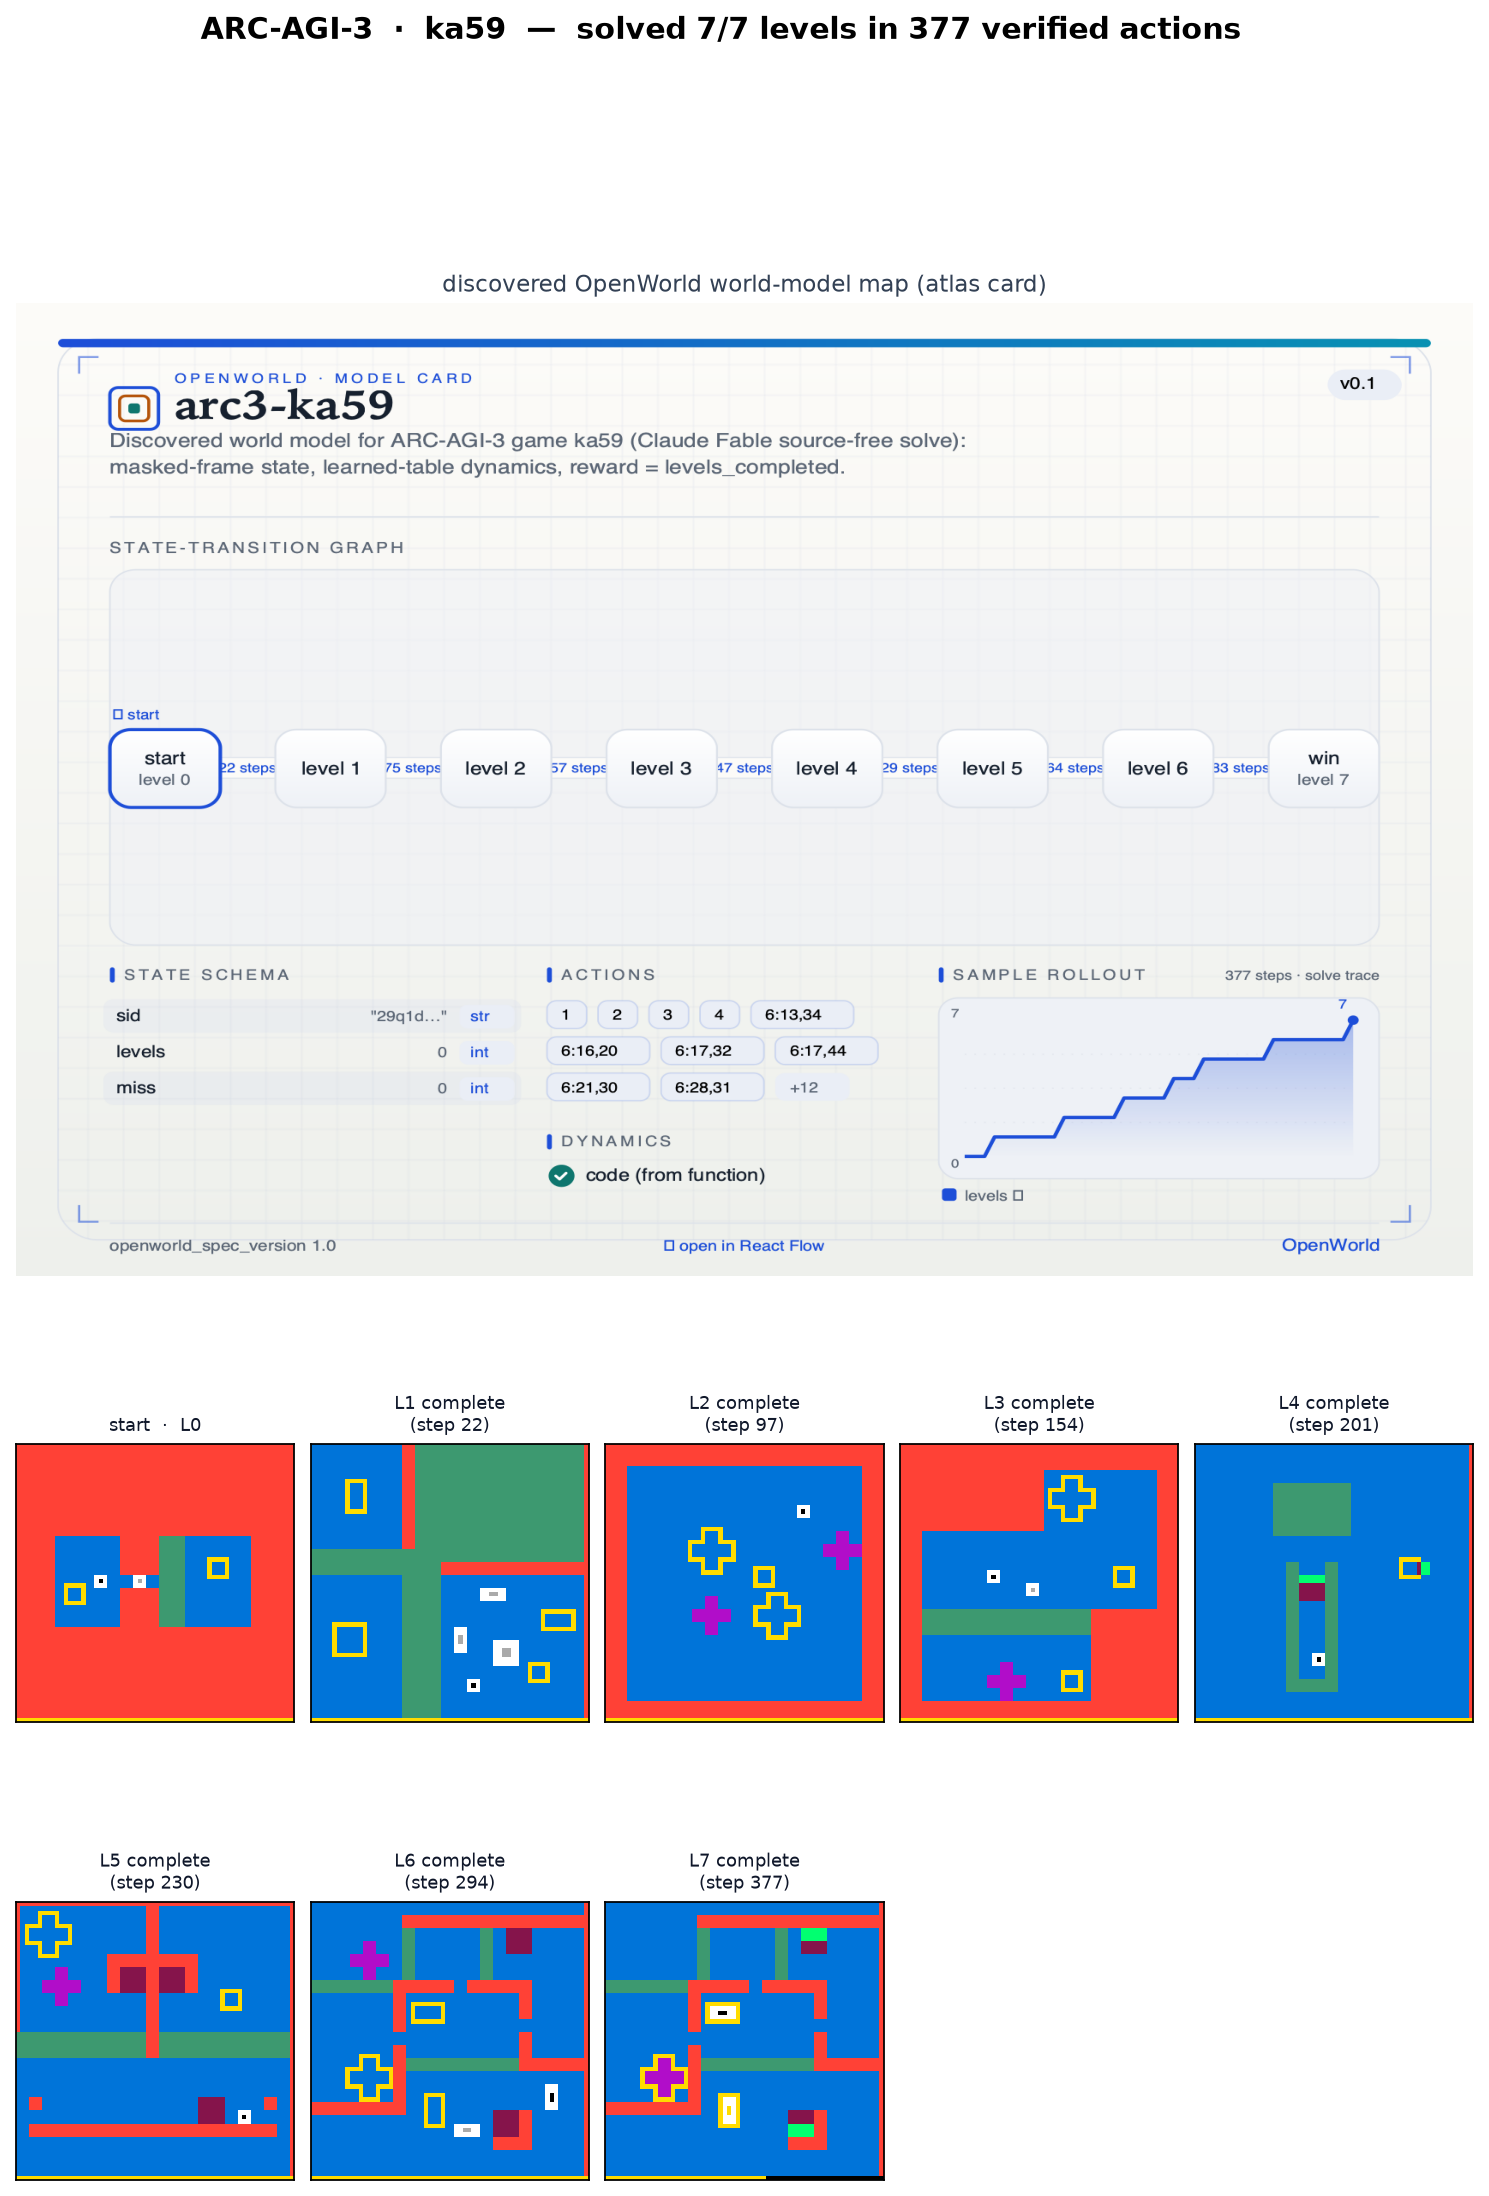
\includegraphics[width=\linewidth,height=0.48\textheight,keepaspectratio]{arc3_replay_ka59.png}\vskip3pt{\color{owmuted}\footnotesize The world-model card (top) plus the level-by-level replay (bottom)\par}
\flushleft \vskip3pt{\footnotesize \begin{itemize}
  \item The card's map is the path through the levels, with each step's button on it
  \item The replay: real screenshots at each level clear, re-run against the game
\end{itemize}}
\end{frame}
\begin{frame}{Example solve: dc22 (6/6) -- a recipe wall}
\centering
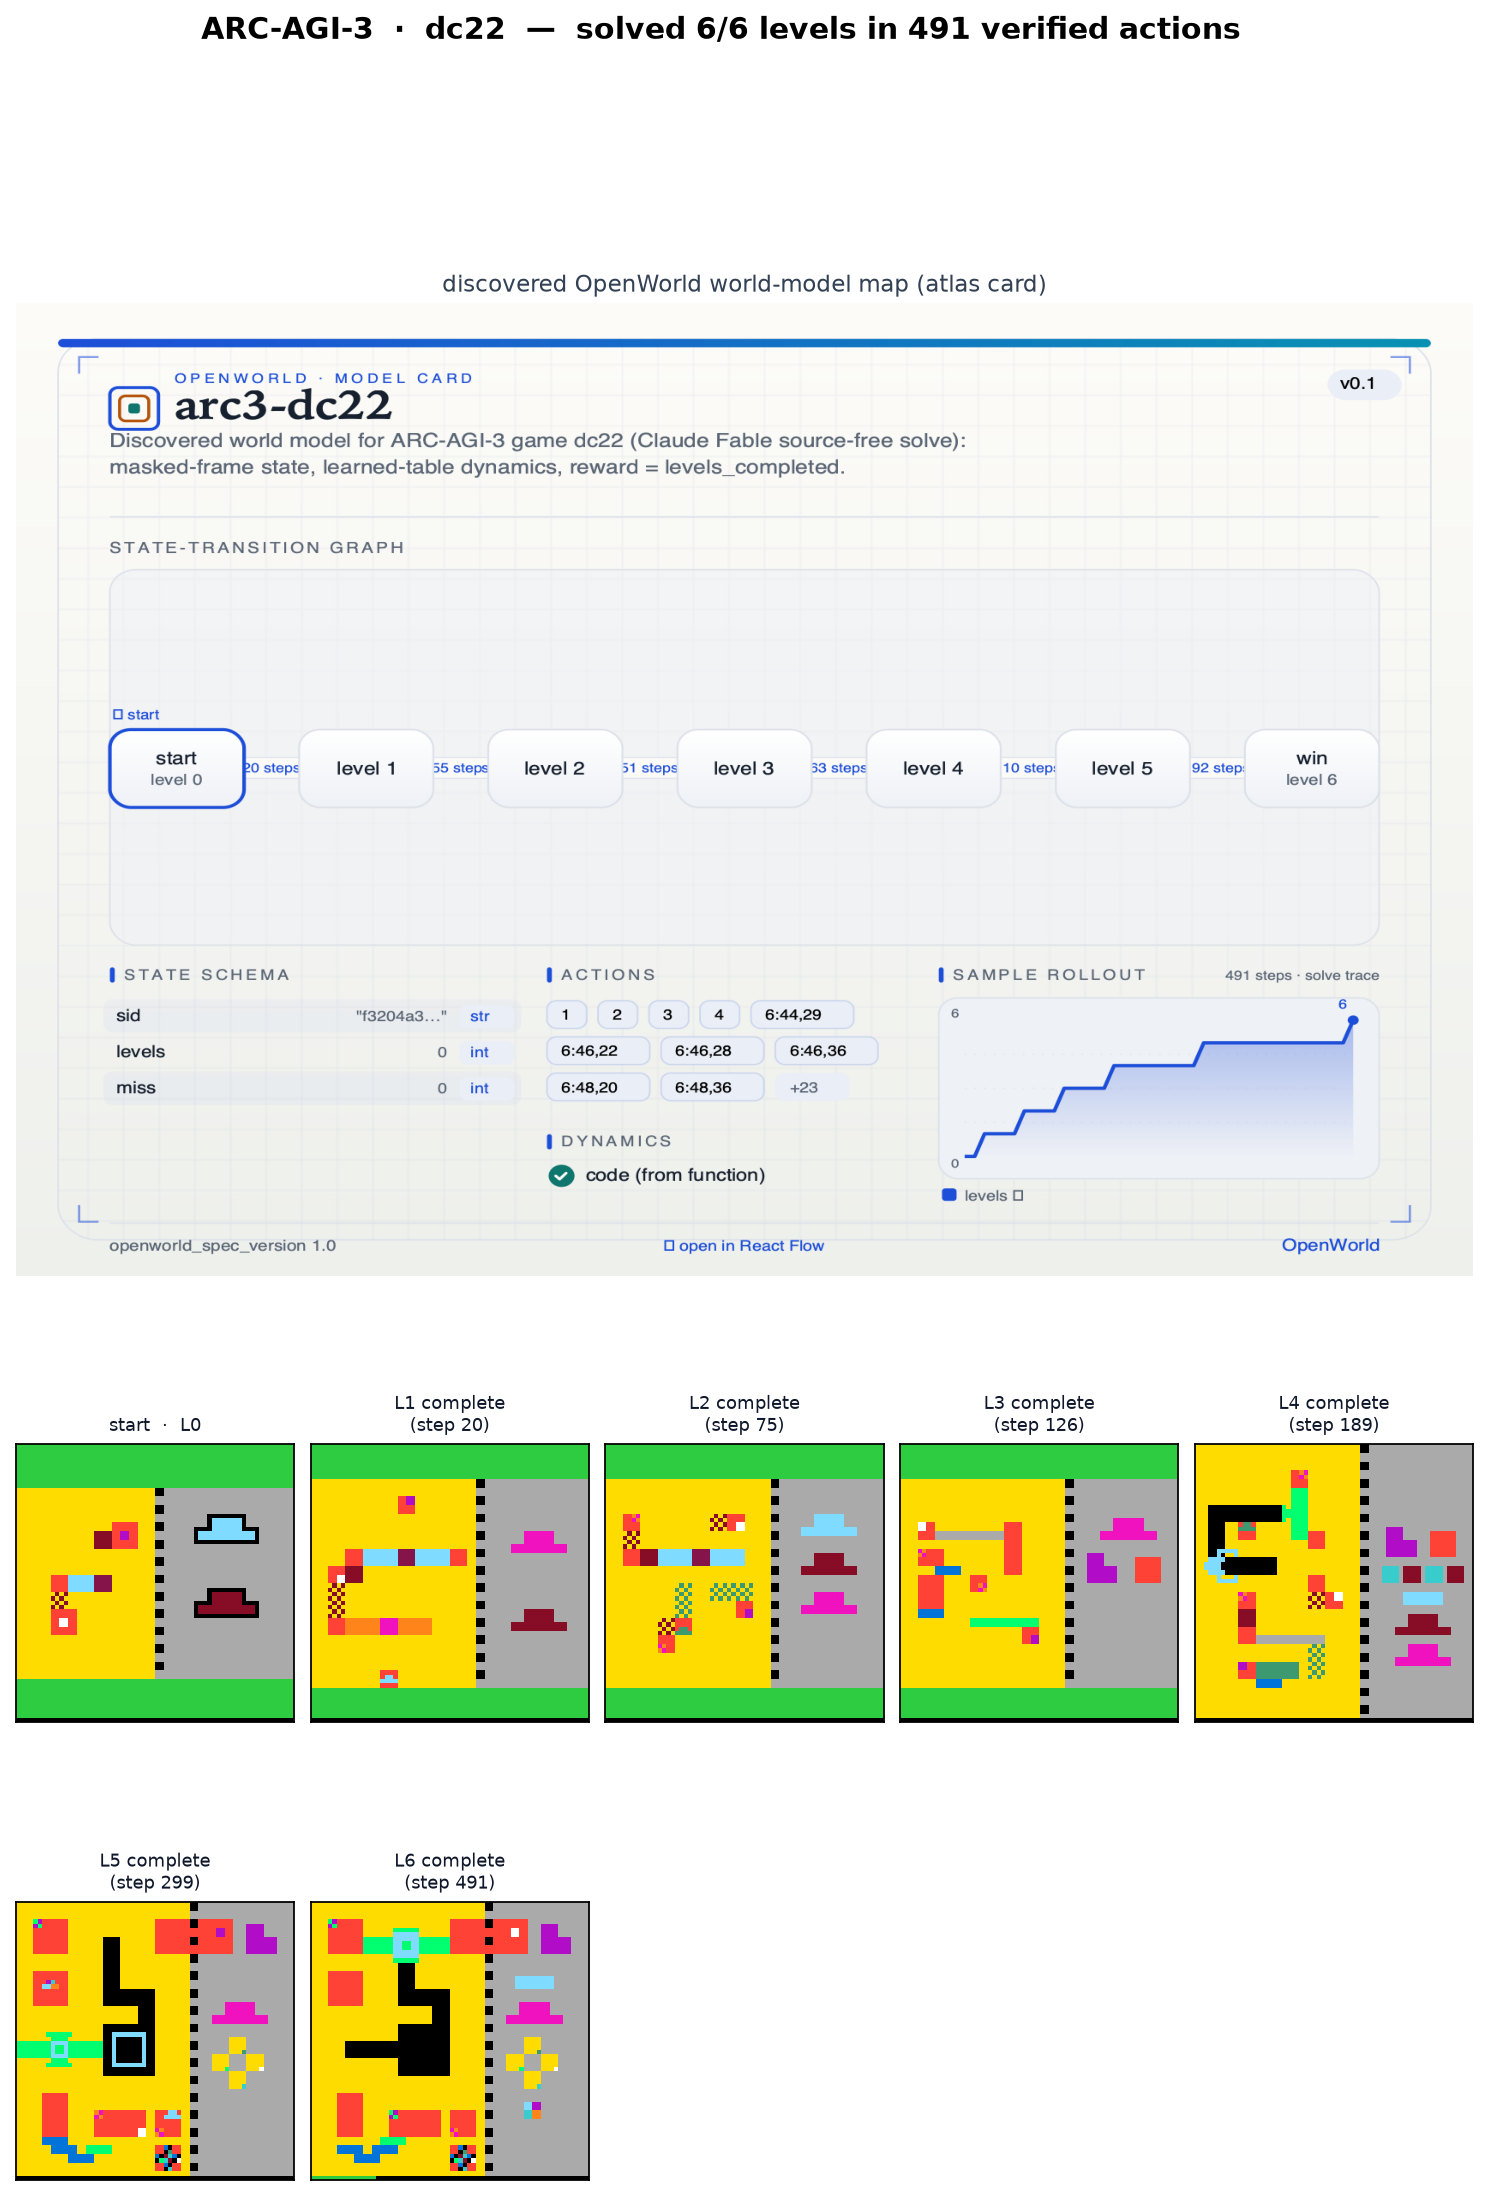
\includegraphics[width=\linewidth,height=0.48\textheight,keepaspectratio]{arc3_replay_dc22.png}\vskip3pt{\color{owmuted}\footnotesize Mixes moving and clicking; only the reasoning agent crosses it\par}
\flushleft \vskip3pt{\footnotesize \begin{itemize}
  \item Random play never even reaches level 1 here
  \item A key-and-box routine slides a movable structure into place
\end{itemize}}
\end{frame}
\begin{frame}{Example solve: g50t (7/7) -- ghost-switch}
\centering
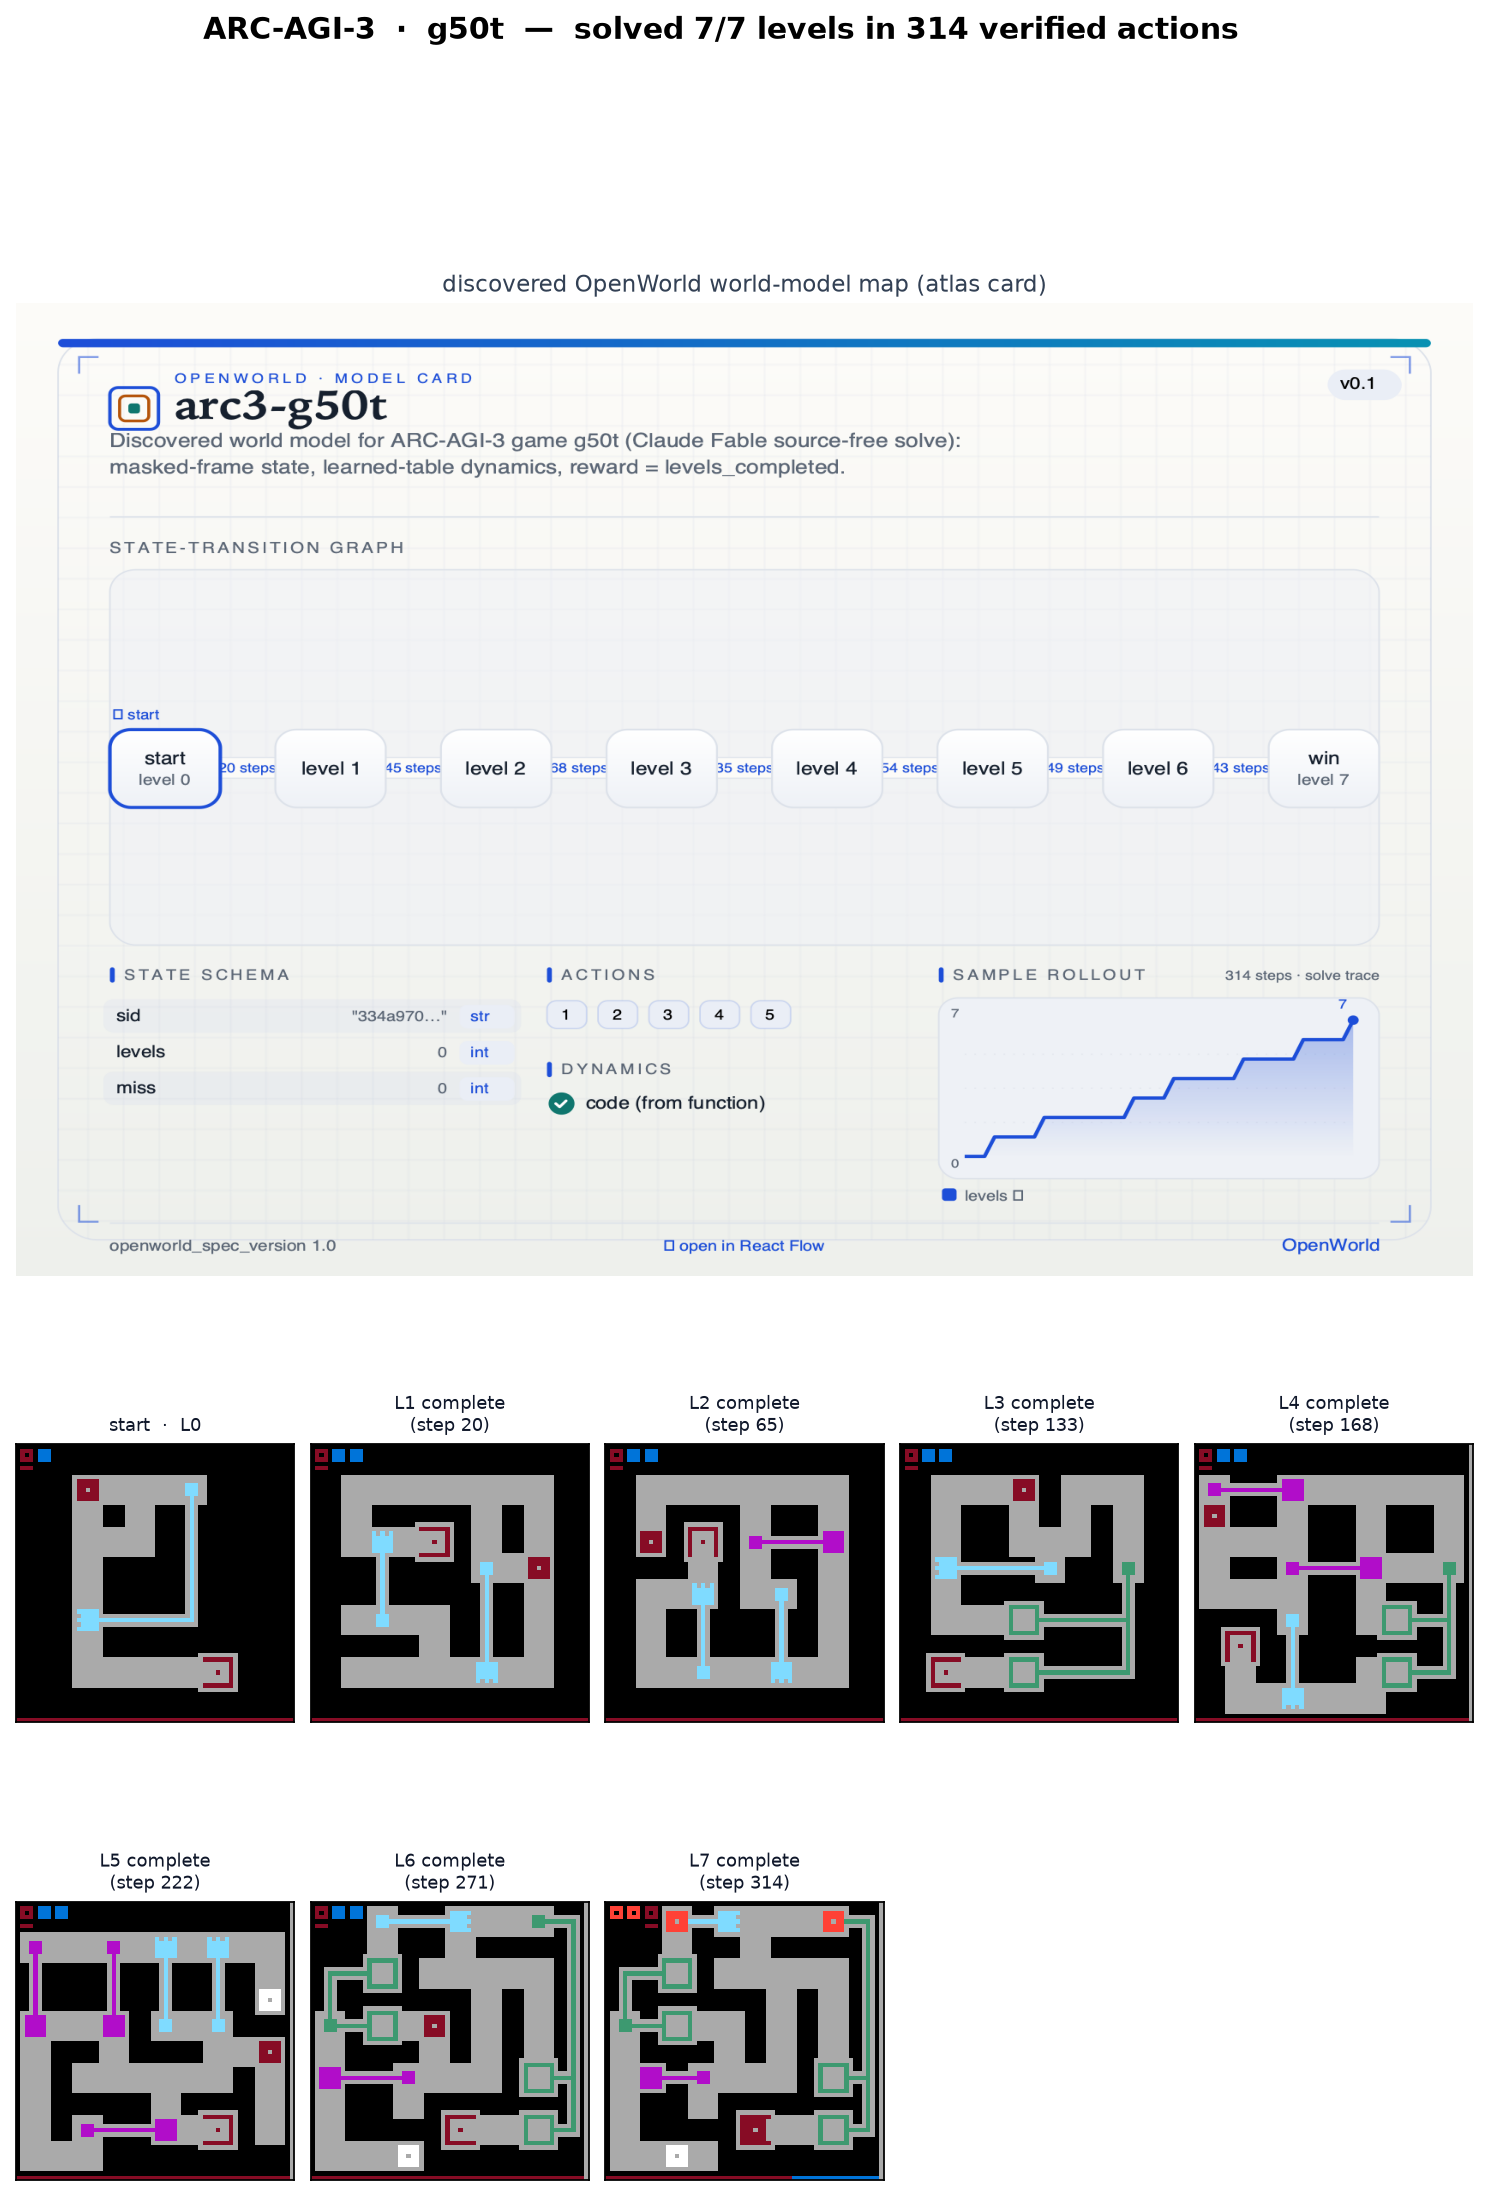
\includegraphics[width=\linewidth,height=0.48\textheight,keepaspectratio]{arc3_replay_g50t.png}\vskip3pt{\color{owmuted}\footnotesize A big 94-spot map never proves a win on its own -- reasoning is what does it\par}
\flushleft \vskip3pt{\footnotesize \begin{itemize}
  \item Hold-down plates, toggle buttons, warp rings, a pinball ghost that copies you
  \item The value is the proven winning chain, not how big the map is
\end{itemize}}
\end{frame}
\begin{frame}{The last wall: lf52 (10/10)}
\centering
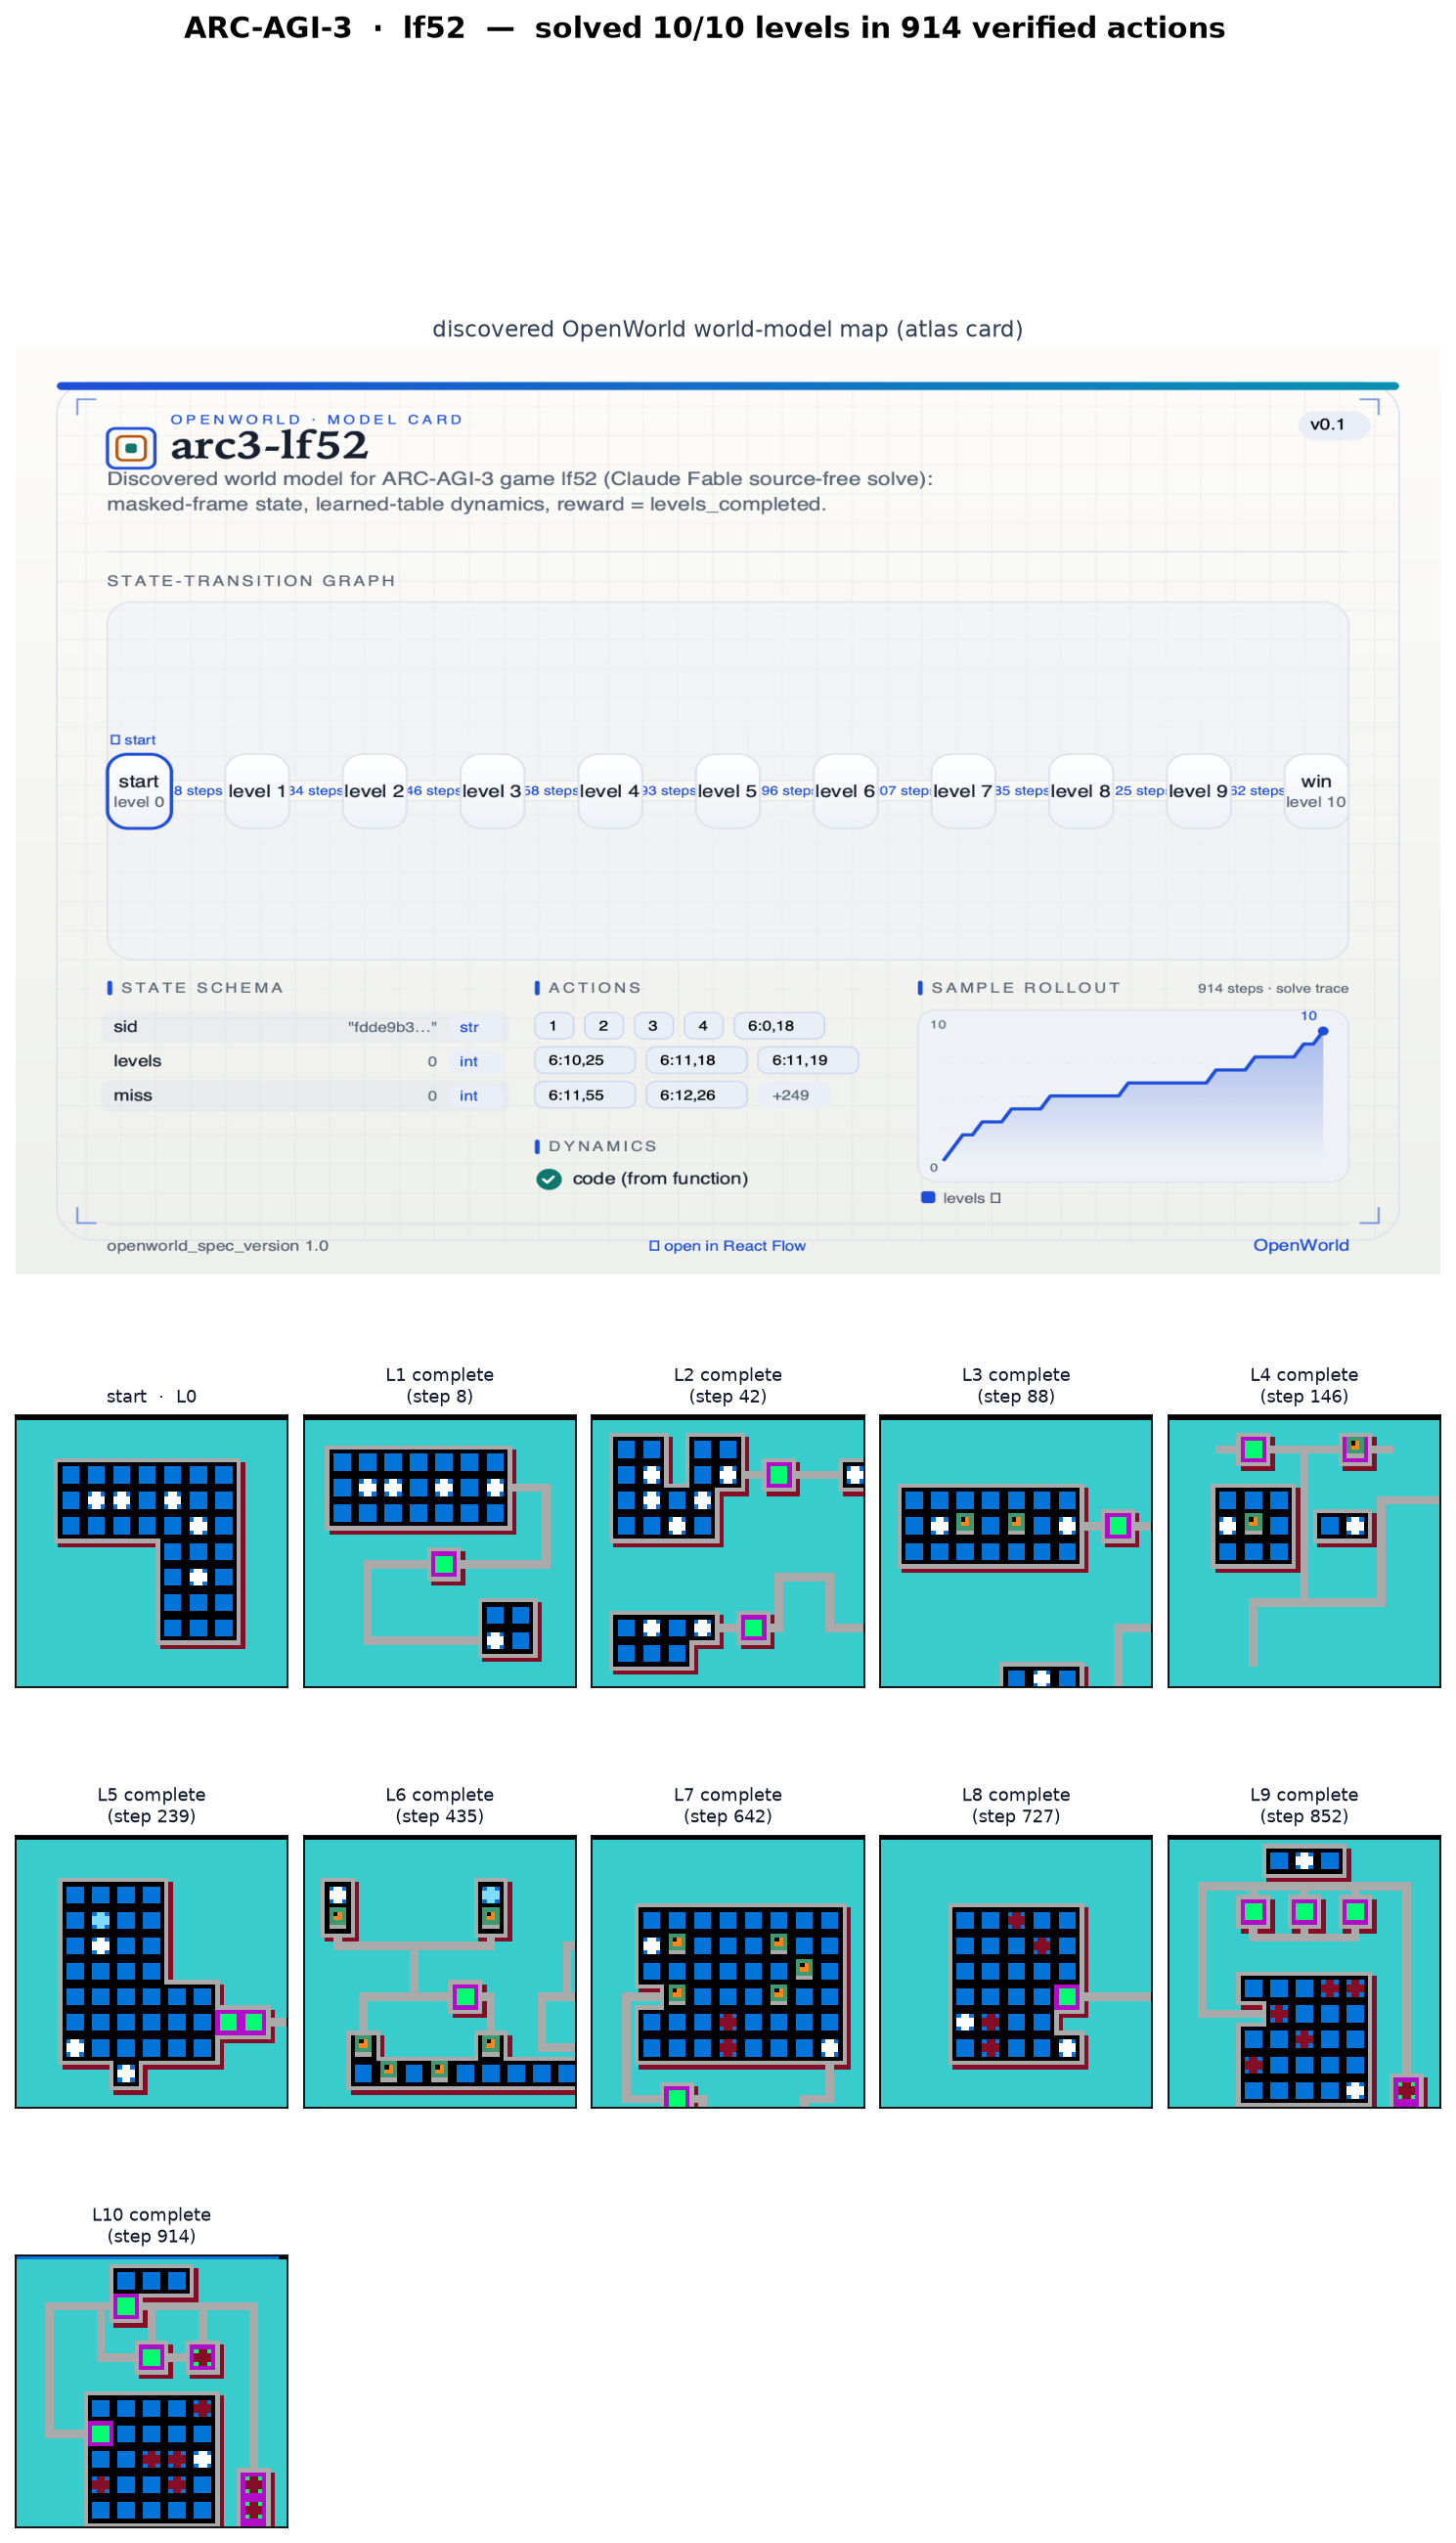
\includegraphics[width=\linewidth,height=0.48\textheight,keepaspectratio]{arc3_replay_lf52.png}\vskip3pt{\color{owmuted}\footnotesize The one level no run had ever solved -- a proven 914-move path\par}
\flushleft \vskip3pt{\footnotesize \begin{itemize}
  \item Cracked with a keep-your-notes deep-wall routine
  \item Build a proven copy of the level, then search it offline at full scale
  \item Solving it completed the perfect 25/25 sweep
\end{itemize}}
\end{frame}
\begin{frame}{Example solve: su15 (9/9) -- merge and deliver}
\centering
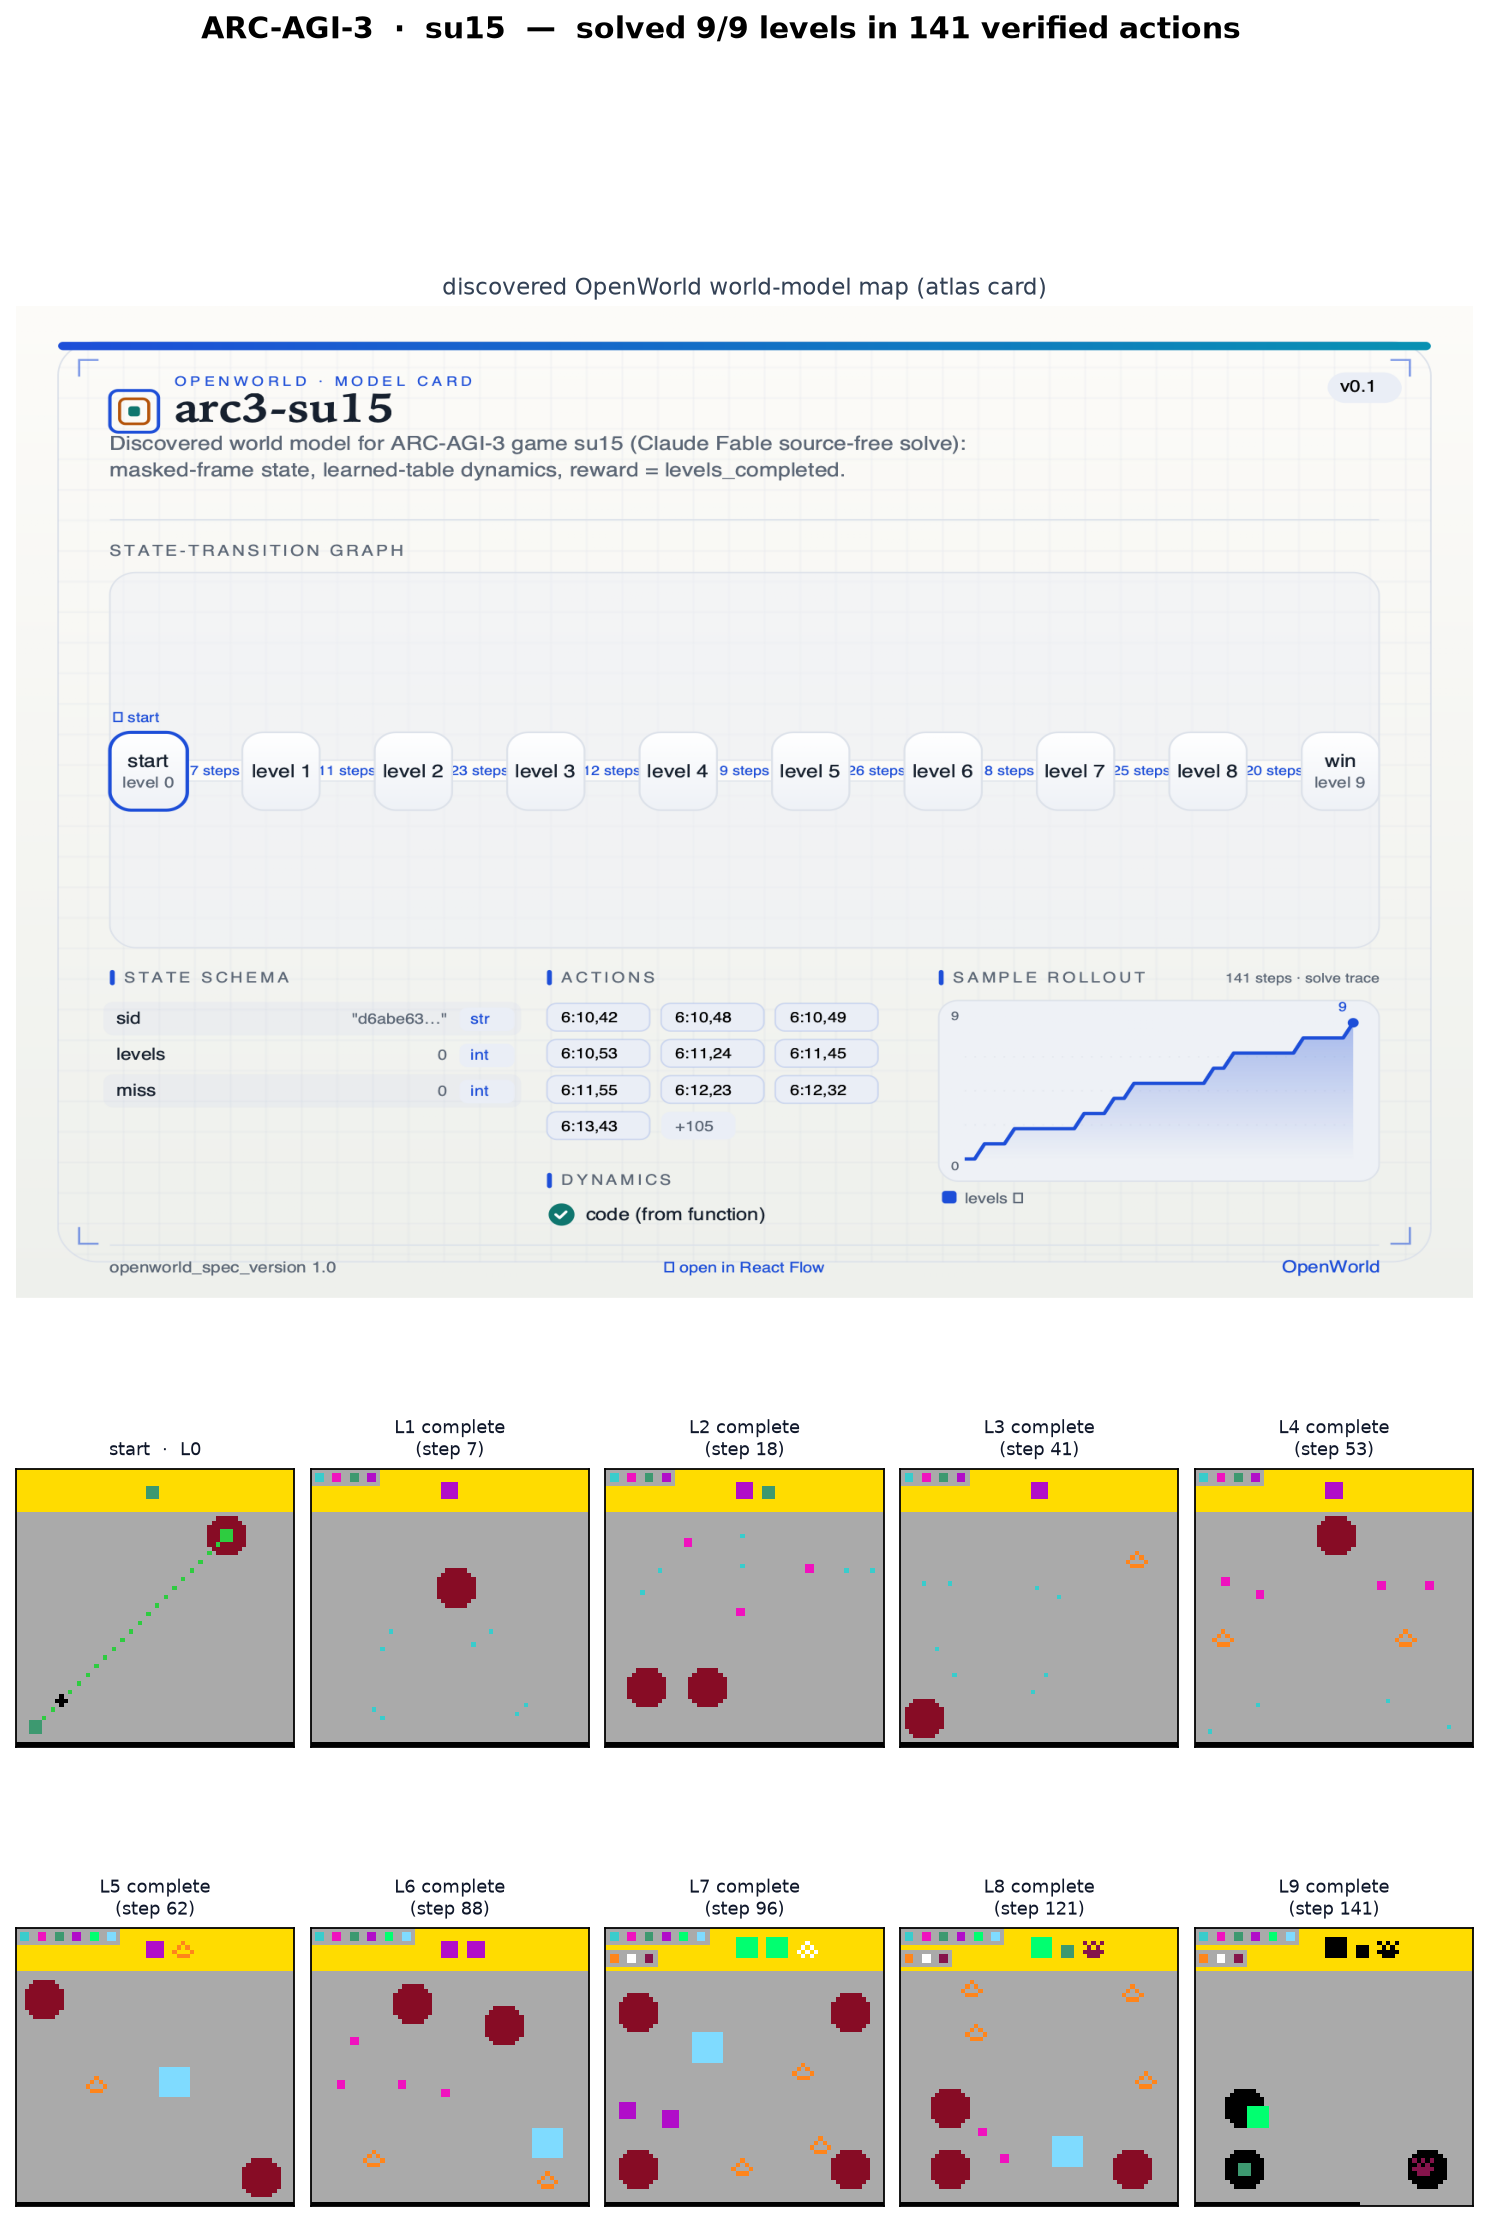
\includegraphics[width=\linewidth,height=0.48\textheight,keepaspectratio]{arc3_replay_su15.png}\vskip3pt{\color{owmuted}\footnotesize Click to gather; matching tiers merge and grow; a 141-click solution\par}
\flushleft \vskip3pt{\footnotesize \begin{itemize}
  \item The clickable targets were figured out from the pixels alone
  \item Runs as a real, openable OpenWorld world
\end{itemize}}
\end{frame}
\begin{frame}[plain]\centering\vfill
{\color{owochre}\rule{40pt}{2.5pt}}\par\vskip10pt
{\color{owdeep}\bfseries\Large How the models actually solve (the play-by-play)\par}\vfill\end{frame}
\begin{frame}{The shape of a solve}
\centering
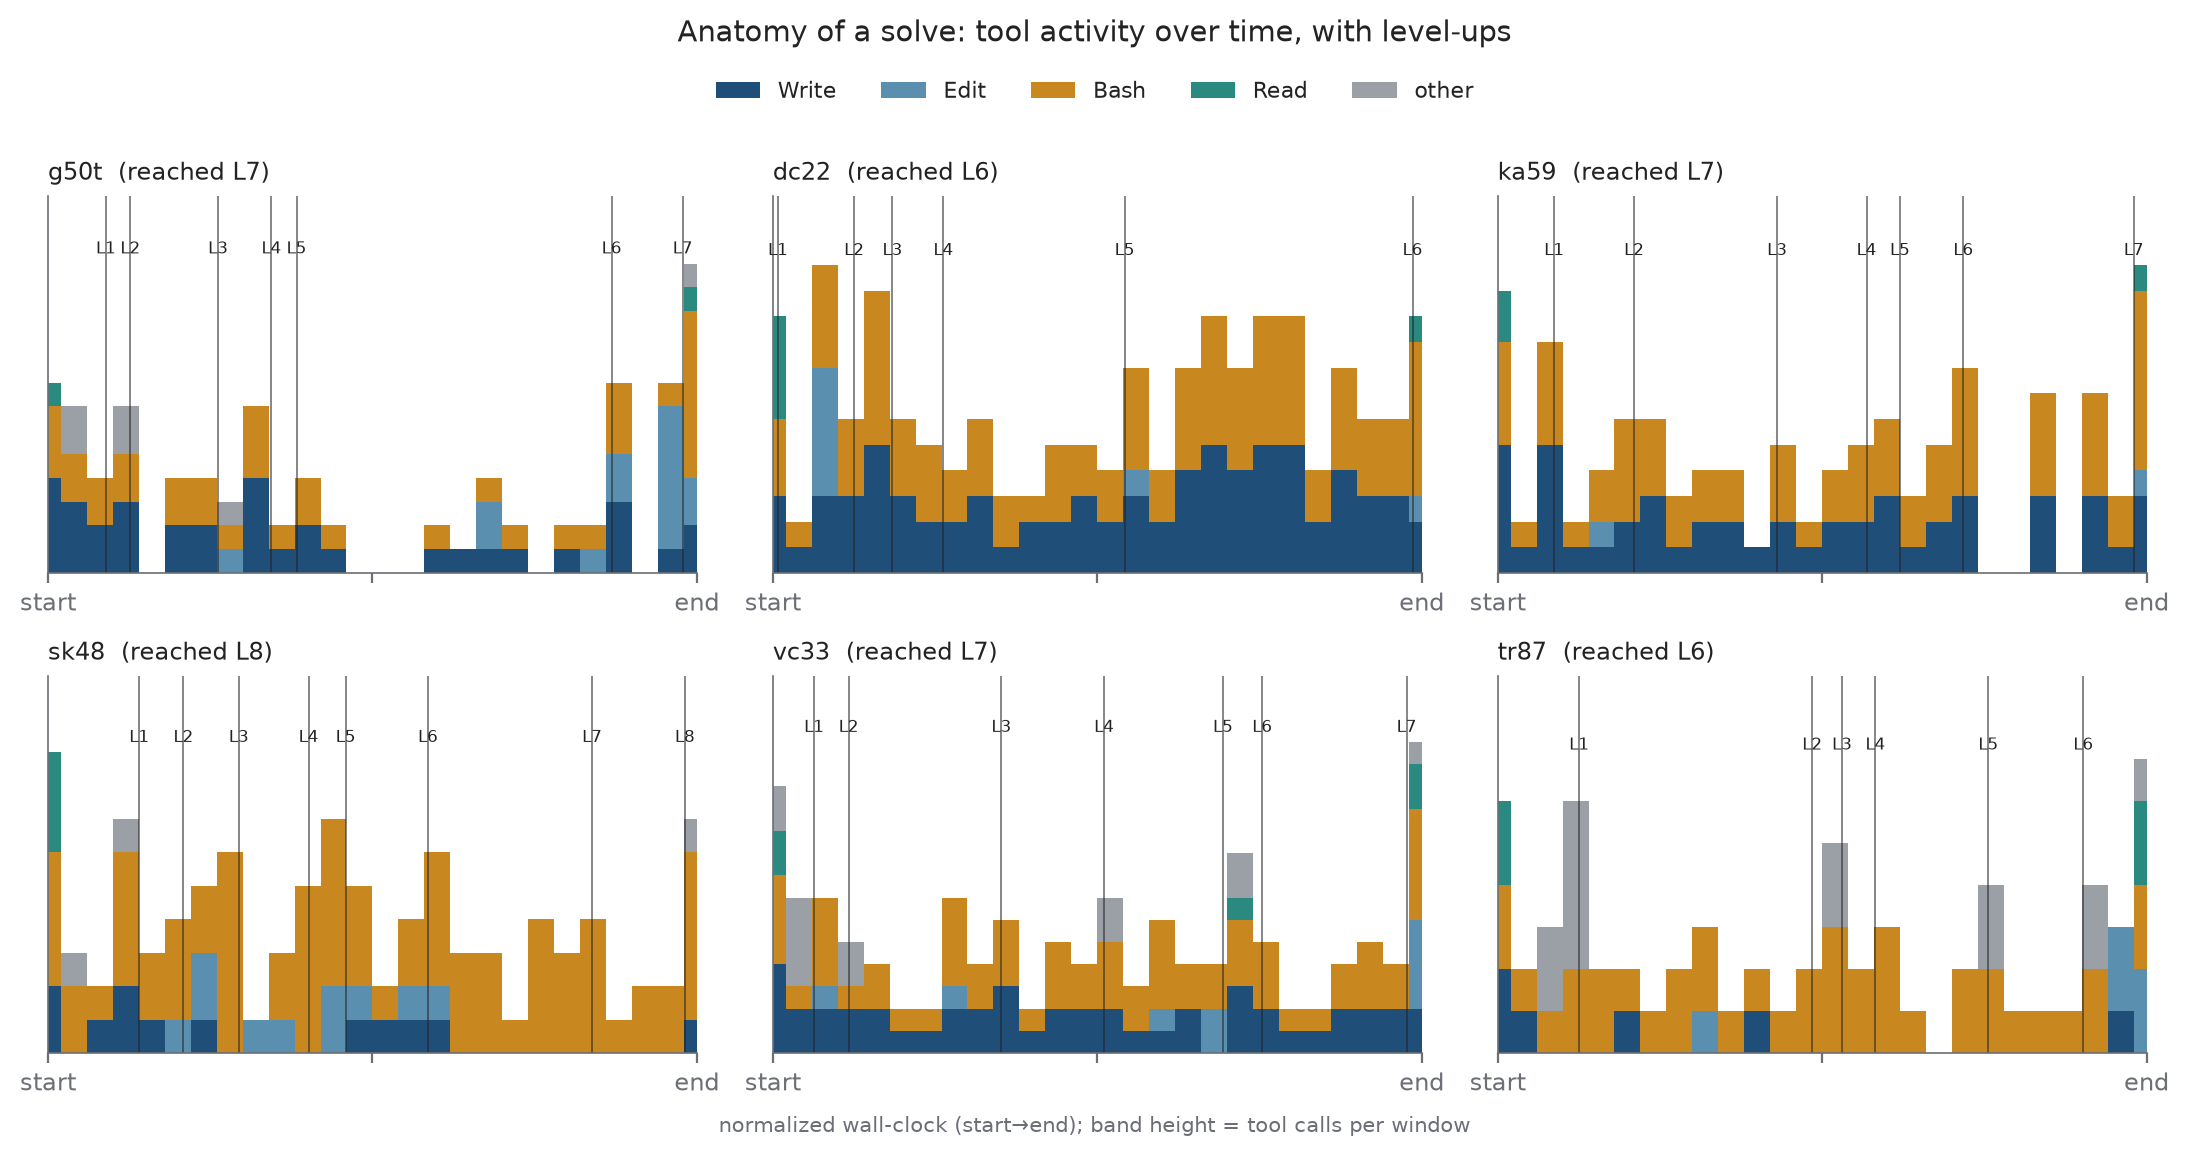
\includegraphics[width=\linewidth,height=0.48\textheight,keepaspectratio]{e150_cardiogram.png}\vskip3pt{\color{owmuted}\footnotesize Read/Write-heavy start (building) -> Bash-heavy middle (searching) -> Edit fixes\par}
\flushleft \vskip3pt{\footnotesize \begin{itemize}
  \item Levels get cleared in sudden jumps, not steady progress
  \item Build first, then search -- the same shape in every solve
\end{itemize}}
\end{frame}
\begin{frame}{The words each game made the agent invent}
\centering
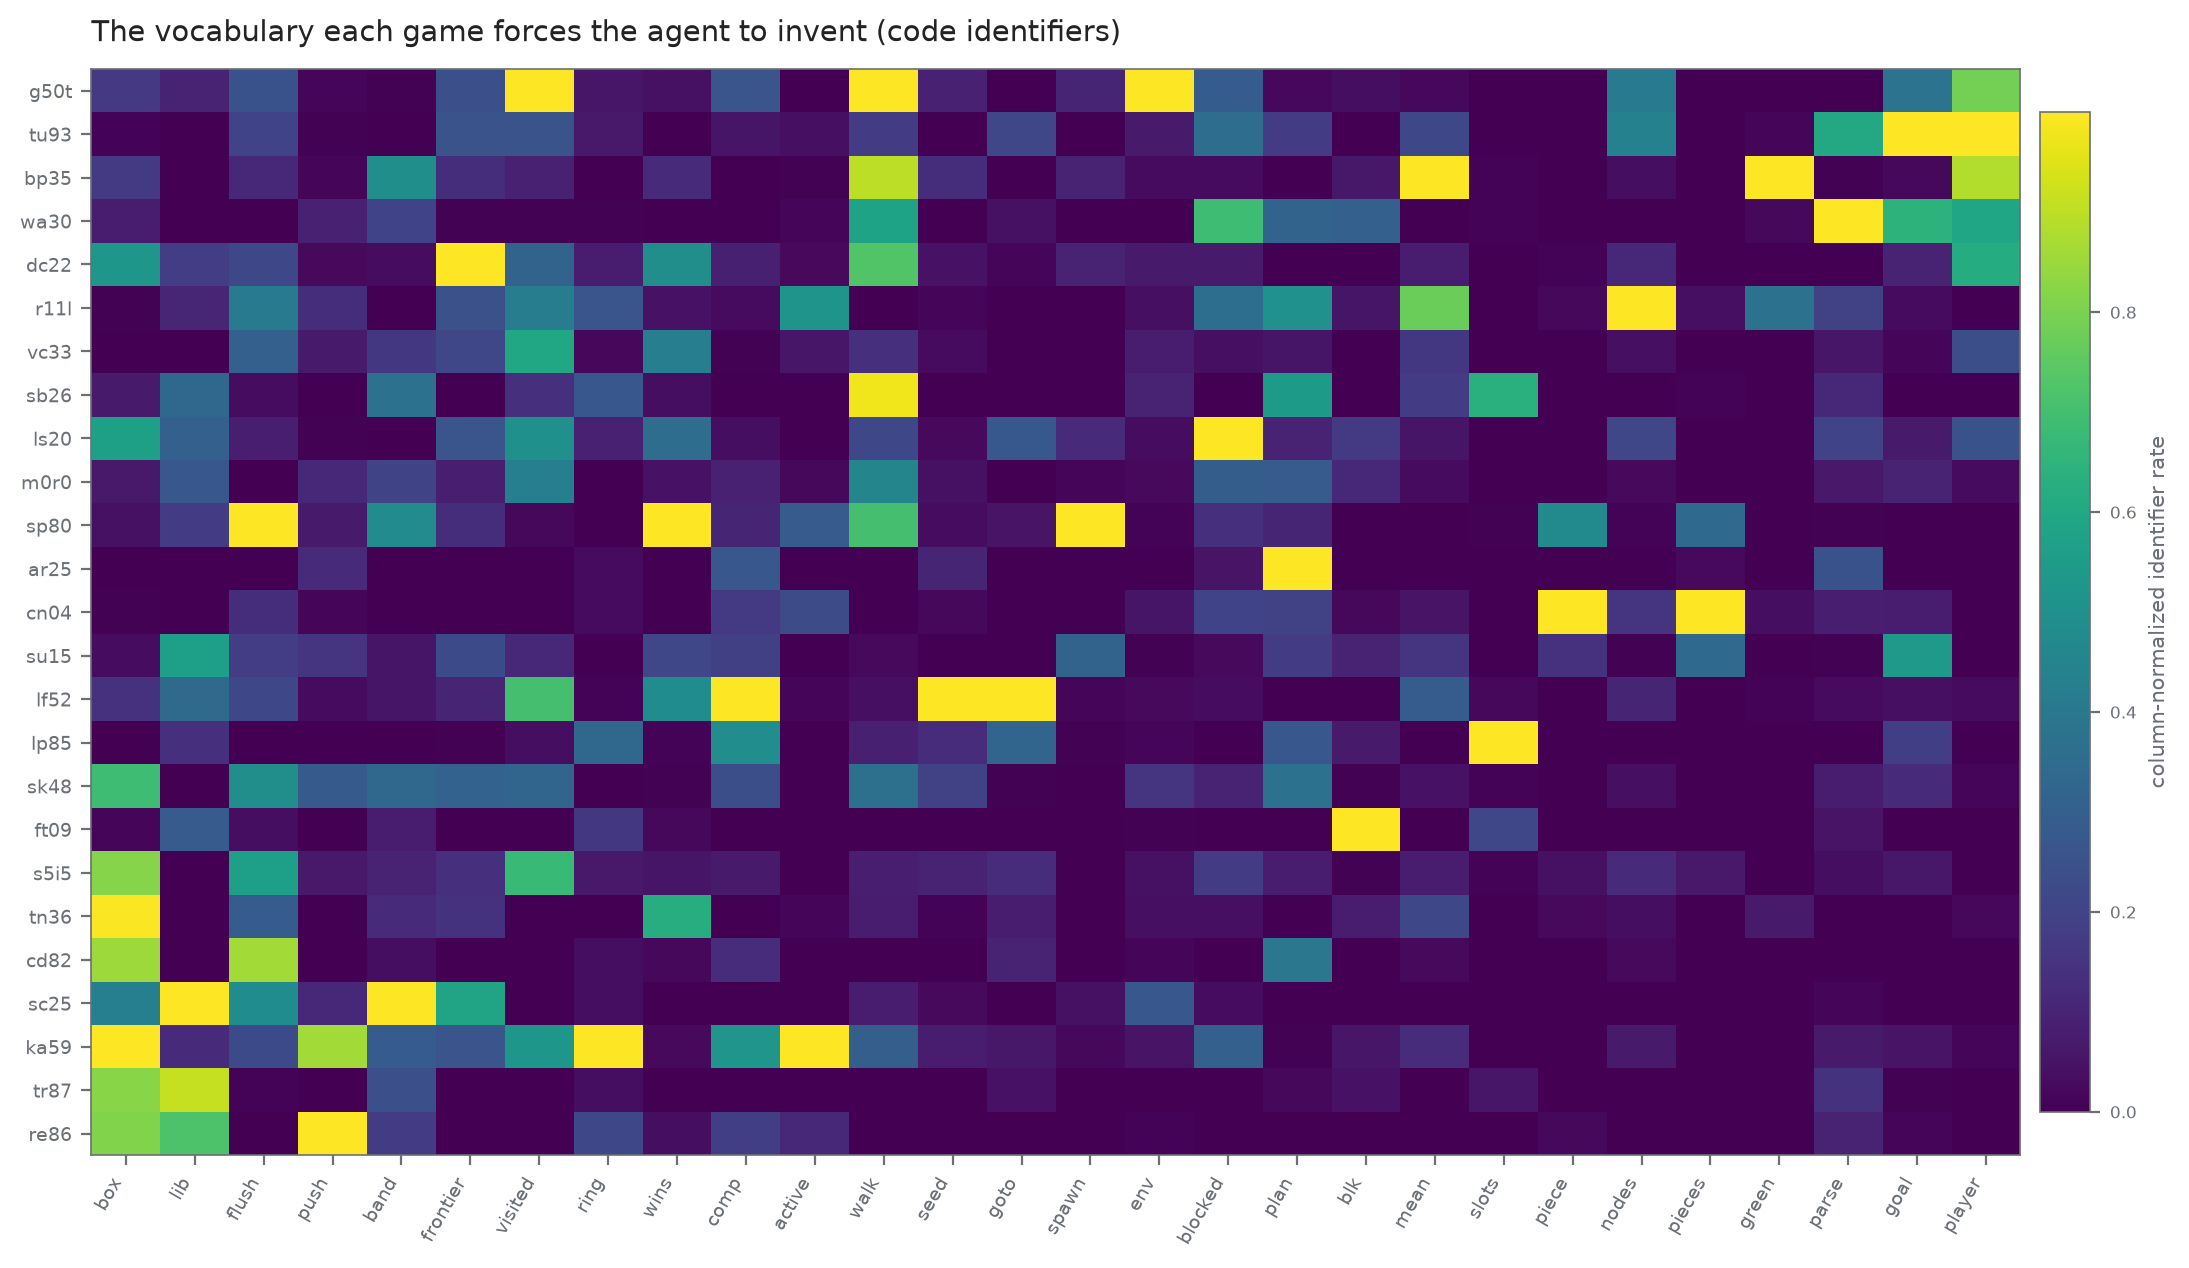
\includegraphics[width=\linewidth,height=0.48\textheight,keepaspectratio]{e150_concepts.png}\vskip3pt{\color{owmuted}\footnotesize The names the agent chose in its code recover each game's mechanics, with no help\par}
\flushleft \vskip3pt{\footnotesize \begin{itemize}
  \item ka59 -> box/push/ring (box-pushing); ft09 -> blk/slots (stencil)
  \item The ideas the agent had to invent tell you what kind of puzzle it was
\end{itemize}}
\end{frame}
\begin{frame}{The signature of each solution}
\centering
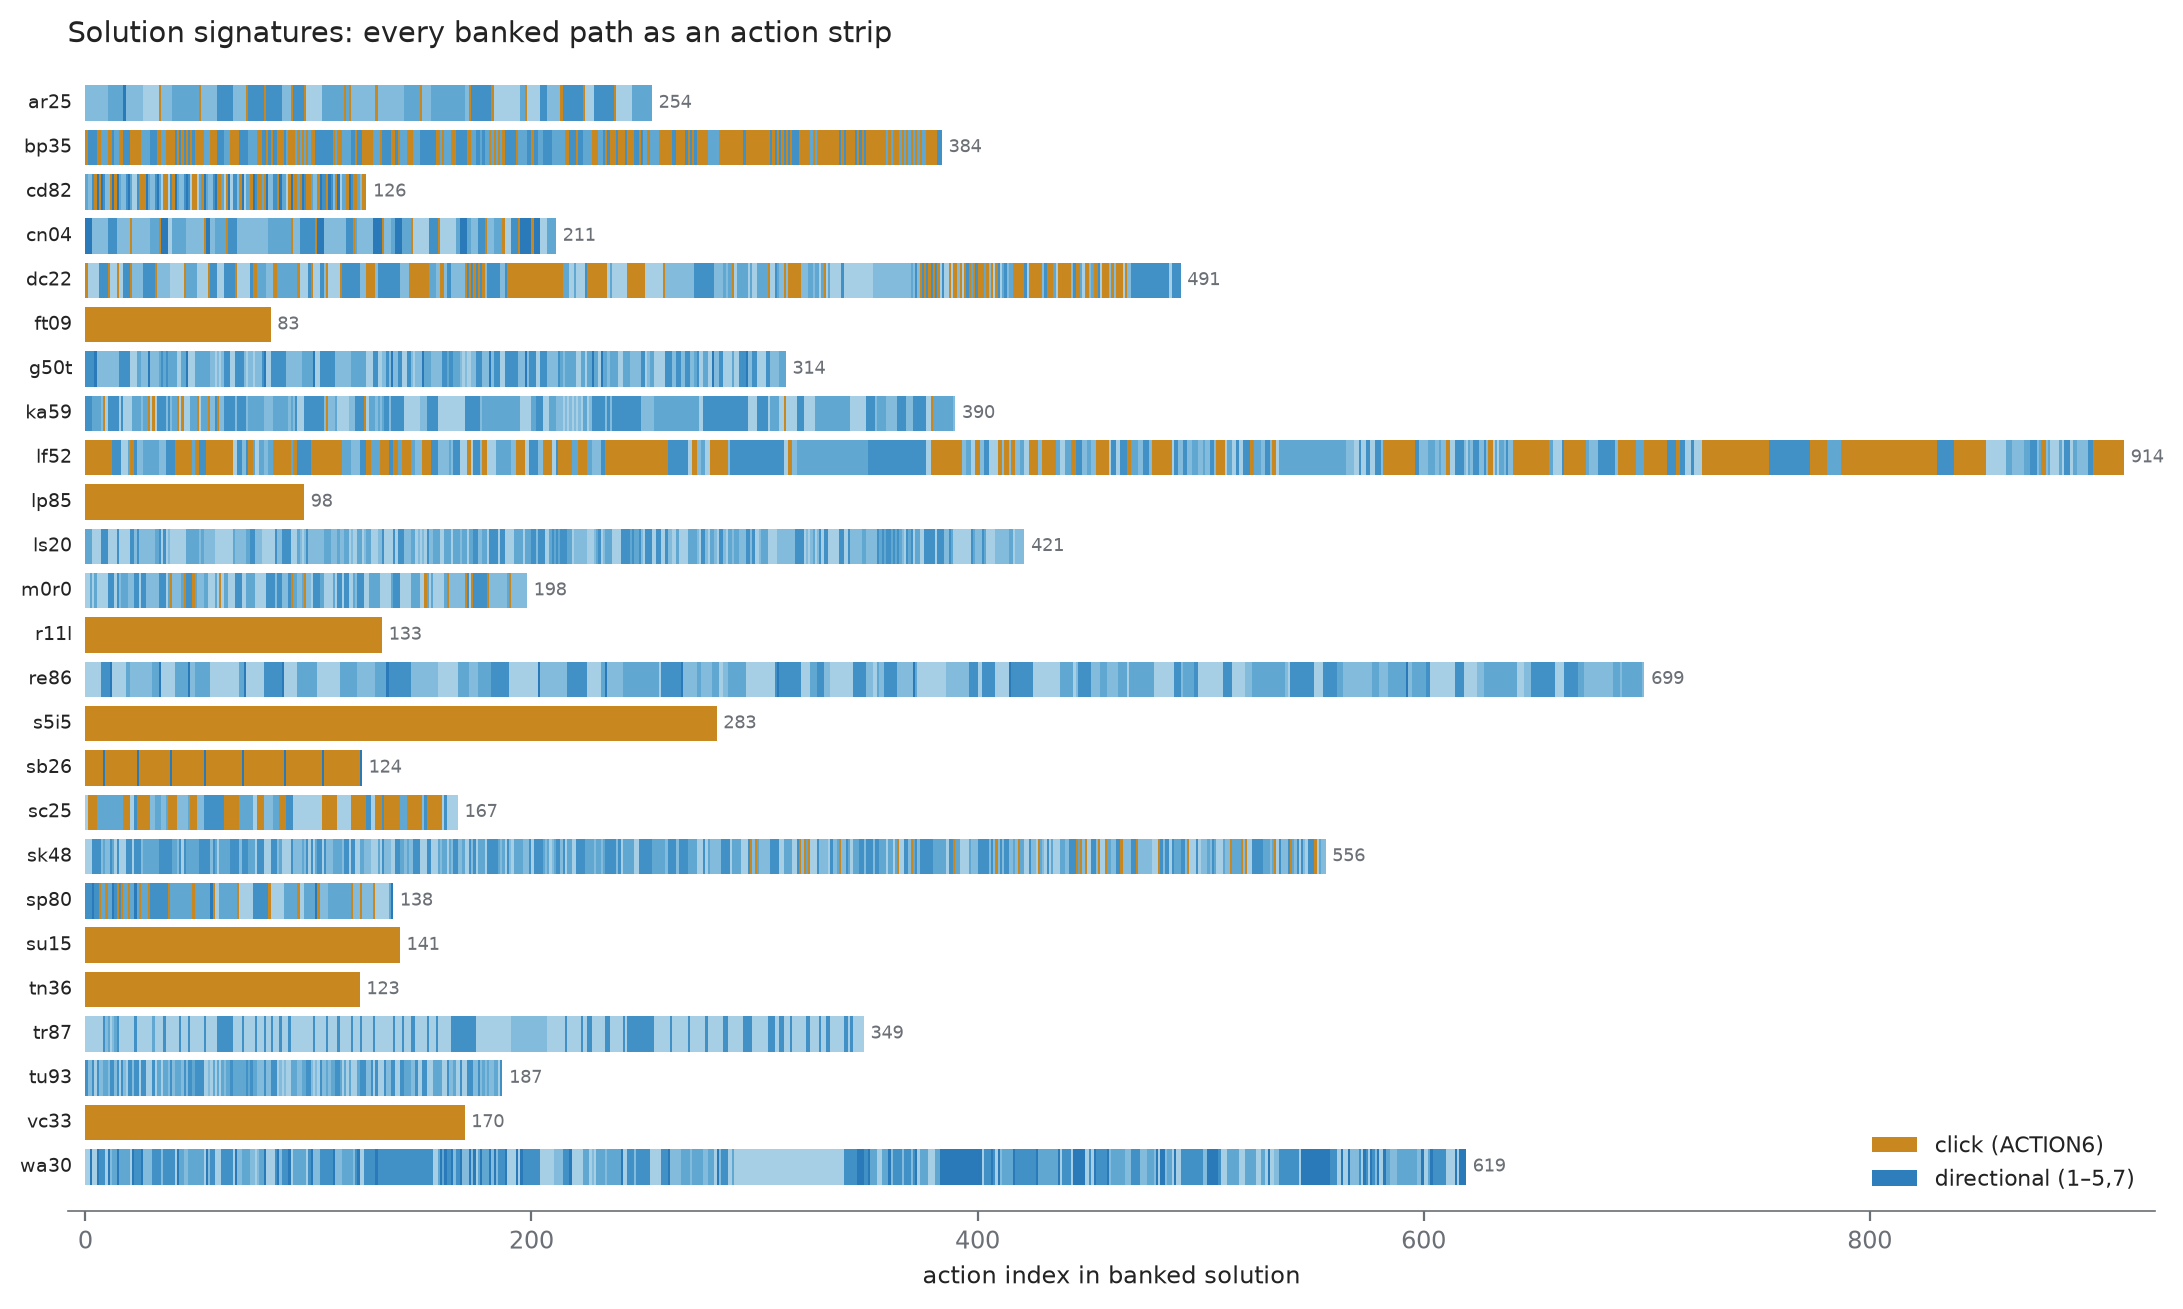
\includegraphics[width=\linewidth,height=0.48\textheight,keepaspectratio]{e150_signatures.png}\vskip3pt{\color{owmuted}\footnotesize Each winning path as a strip of moves: clicks, moving, or a mix\par}
\flushleft \vskip3pt{\footnotesize \begin{itemize}
  \item Ochre = click (ACTION6); blue = moving (1-5,7)
  \item A picture-map of each solution's shape and length (lf52 is longest)
\end{itemize}}
\end{frame}
\begin{frame}{Where the agent clicked}
\centering
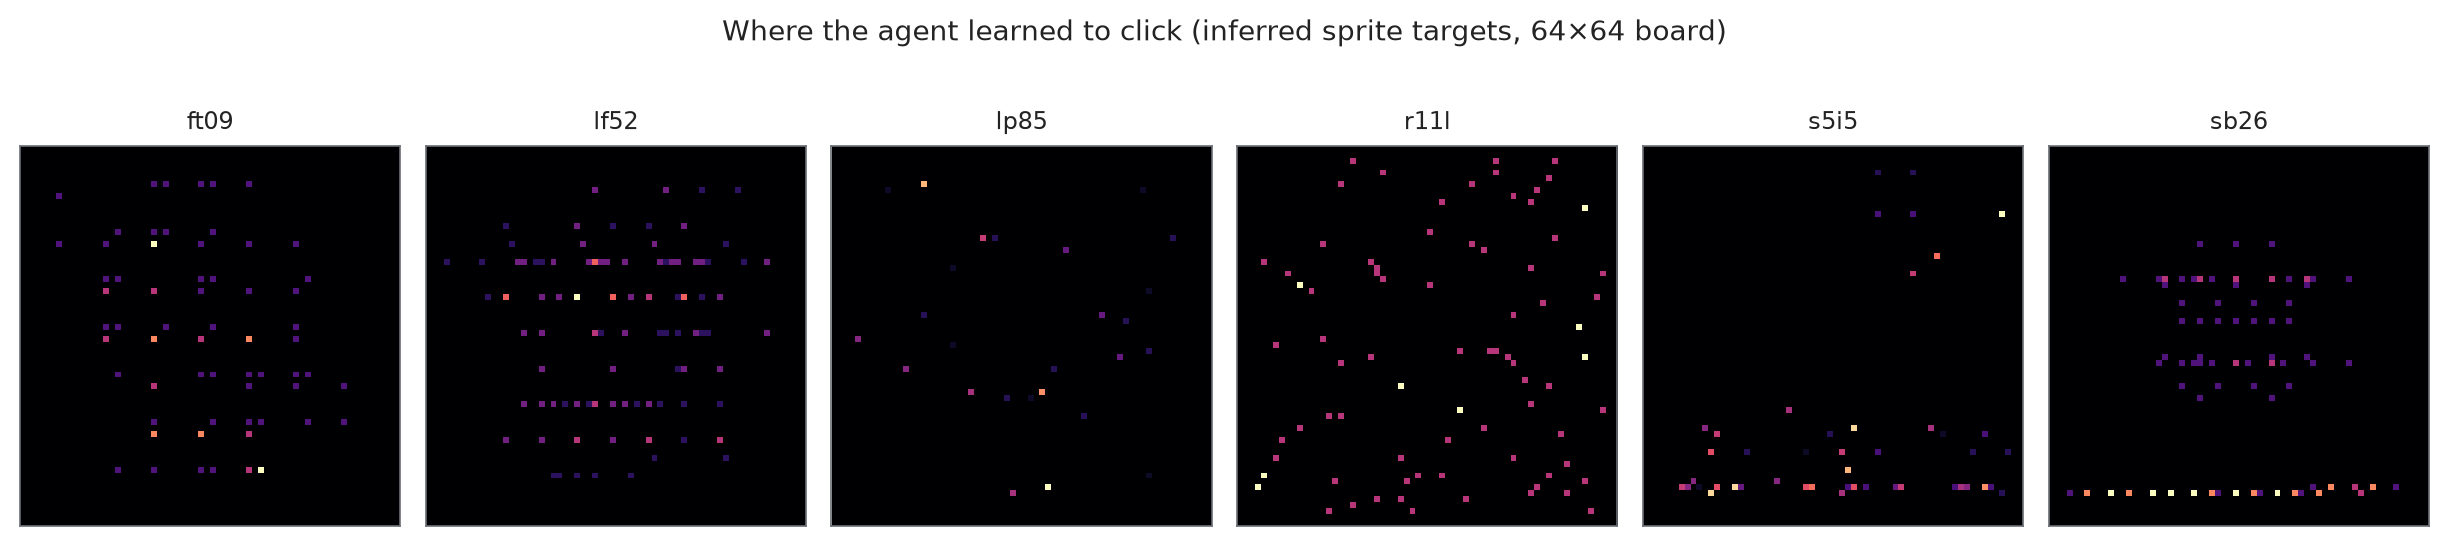
\includegraphics[width=\linewidth,height=0.48\textheight,keepaspectratio]{e150_clicks.png}\vskip3pt{\color{owmuted}\footnotesize How thick the winning clicks land on the 64x64 board -- no hidden list of targets\par}
\flushleft \vskip3pt{\footnotesize \begin{itemize}
  \item The clickable spots the agent figured out from the pixels alone
  \item opus looks harder at the picture; Fable leans on memory plus checking
\end{itemize}}
\end{frame}
\begin{frame}[plain]\vfill\centering \resizebox{0.95\textwidth}{!}{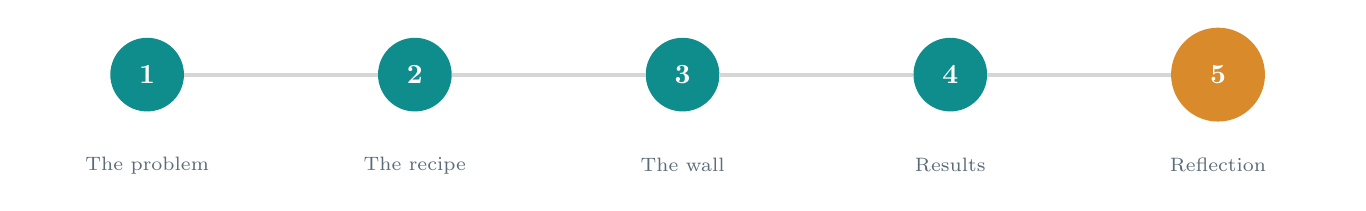
\begin{tikzpicture}[stn/.style={circle,draw=owteal,line width=1pt,minimum size=9mm,font=\bfseries,inner sep=0,text=owteal},std/.style={circle,draw=owteal,fill=owteal,line width=1pt,minimum size=9mm,font=\bfseries,inner sep=0,text=white},stc/.style={circle,draw=owochre,fill=owochre,line width=1.2pt,minimum size=11.5mm,font=\bfseries,inner sep=0,text=white},stx/.style={circle,draw=owmuted,line width=1pt,minimum size=9mm,font=\bfseries,inner sep=0,text=owmuted},stlbl/.style={font=\scriptsize,text=owmuted,align=center,text width=28mm},stln/.style={draw=black!16,line width=1.4pt}]\node[std] (s0) at (0.0,0) {1};\node[std] (s1) at (3.4,0) {2};\node[std] (s2) at (6.8,0) {3};\node[std] (s3) at (10.2,0) {4};\node[stc] (s4) at (13.6,0) {5};\node[stlbl] at (0.0,-1.15) {The problem};\node[stlbl] at (3.4,-1.15) {The recipe};\node[stlbl] at (6.8,-1.15) {The wall};\node[stlbl] at (10.2,-1.15) {Results};\node[stlbl] at (13.6,-1.15) {Reflection};\draw[stln] (s0)--(s1);\draw[stln] (s1)--(s2);\draw[stln] (s2)--(s3);\draw[stln] (s3)--(s4);\end{tikzpicture}}\\[24pt]
{\color{owochre}\bfseries\footnotesize PART 5}\\[5pt]
{\color{owdeep}\bfseries\Large Reflection}\\[10pt]{\color{owmuted}\large Honest limits and what comes next}\vfill\end{frame}
\begin{frame}{It is the best of many tries; a single try is not reliable}\vfill\begin{columns}[c]\begin{column}{0.323\textwidth}\centering{\color{owdeep}\fontsize{40}{44}\selectfont\bfseries \textasciitilde{}823}\\[6pt]{\color{owmuted}\small sessions across 25 games (about 33 per game)}\end{column}\begin{column}{0.323\textwidth}\centering{\color{owochre}\fontsize{40}{44}\selectfont\bfseries \textasciitilde{}6\%}\\[6pt]{\color{owmuted}\small a full win on \textasciitilde{}6\% of tries overall, as low as \textasciitilde{}2\% on bp35/lf52}\end{column}\begin{column}{0.323\textwidth}\centering{\color{owdeep}\fontsize{40}{44}\selectfont\bfseries >1 seed}\\[6pt]{\color{owmuted}\small a clean fixed-prompt, many-seed test is a clear next step}\end{column}\end{columns}\vfill\end{frame}
\begin{frame}{We cannot yet measure if the model saw these games in training}\vfill\begin{columns}[T]\begin{column}{.46\textwidth}{\color{owdeep}\bfseries Code never read}\\[2pt]{\color{owmuted}\small We check that no run reads the game's code -- measured every run}\end{column}\begin{column}{.46\textwidth}{\color{owdeep}\bfseries Memory unknown}\\[2pt]{\color{owmuted}\small But we cannot rule out a public game already sitting in the model's memory}\end{column}\end{columns}\vskip12pt\begin{columns}[T]\begin{column}{.46\textwidth}{\color{owdeep}\bfseries Applies to all}\\[2pt]{\color{owmuted}\small This applies to every top-model result, the earlier best included}\end{column}\begin{column}{.46\textwidth}{\color{owdeep}\bfseries 0/25 by name}\\[2pt]{\color{owmuted}\small Fable knew 0/25 games from the name alone (a quick check, not proof)}\end{column}\end{columns}\vfill\end{frame}
\begin{frame}{Offline, unlimited restarts, one run}\vfill\begin{columns}[c]\begin{column}{.42\textwidth}{\color{owdeep}\large\bfseries What it is}\\[3pt]{\color{owmuted}All solves are offline, with unlimited restarts and perfect replay -- a fresh fair-budget result}\end{column}\begin{column}{.10\textwidth}\begin{center}{\color{owochre}\Huge$\rightarrow$}\end{center}\end{column}\begin{column}{.42\textwidth}{\color{owdeep}\large\bfseries What it is not}\\[3pt]{\color{owmuted}Not the live leaderboard, which docks you for extra moves; a repeat or a live run might change it, and the cost is a rough guess -- the perfect run was not the cheap one}\end{column}\end{columns}\vfill\end{frame}
\begin{frame}[plain]\centering\vfill
{\color{owochre}\rule{40pt}{2.5pt}}\par\vskip10pt
{\color{owdeep}\bfseries\Large Conclusion\par}\vfill\end{frame}
\begin{frame}{What we showed}\vfill\begin{center}{\color{owteal}\fontsize{58}{62}\selectfont\bfseries 25/25}\par\vskip10pt{\color{owdeep}\large first perfect ARC-AGI-3 run, no code ever read (Fable)}\end{center}\vskip10pt\begin{itemize}\item Copying the game is not the wall -- the rules can be written out as code\item The win is a recipe of steps in order; one-screen scoring wins 0\item Only a reasoning agent that writes its own copy crosses it; a stronger model carries it from 16/25 to every game\end{itemize}\vfill\end{frame}
\begin{frame}{The takeaway for builders}\vfill\begin{columns}[T]\begin{column}{0.237\textwidth}{\color{owteal}\rule{20pt}{3pt}}\par\smallskip{\color{owdeep}\bfseries Win = a recipe}\par\smallskip{\small In these games a win is a recipe of steps in order, not one good screen}\end{column}\begin{column}{0.237\textwidth}{\color{owochre}\rule{20pt}{3pt}}\par\smallskip{\color{owdeep}\bfseries Scoring fails}\par\smallskip{\small Any one-screen score fails, even with a perfect copy -- aim at finding the recipe, not scoring screens}\end{column}\begin{column}{0.237\textwidth}{\color{owblue}\rule{20pt}{3pt}}\par\smallskip{\color{owdeep}\bfseries Runnable worlds}\par\smallskip{\small Every solver is an open, replay-proven, runnable world}\end{column}\begin{column}{0.237\textwidth}{\color{owmuted}\rule{20pt}{3pt}}\par\smallskip{\color{owdeep}\bfseries What's next}\par\smallskip{\small Live-run efficiency, many-seed spread, a training-memory-controlled test}\end{column}\end{columns}\vfill\end{frame}
\begin{frame}[plain]\centering\vfill
{\color{owdeep}\bfseries\LARGE The recipe of steps is the wall. Reasoning is the ladder. Every solve downloads, re-runs, and opens as a world.\par}\vfill\end{frame}
\begin{frame}[plain]\centering\vfill{\color{owochre}\rule{40pt}{2.5pt}}\par\vskip12pt{\color{owdeep}\bfseries\Large The code is open --- go star it\par}\vskip16pt
\includegraphics[width=4.2cm]{qr_openworld.png}\par\vskip12pt{\color{owblue}\large github.com/quome-cloud/openworld\par}\vskip4pt{\color{owmuted}\small 100 world recipes \textperiodcentered\ the papers \textperiodcentered\ every experiment\par}\vfill\end{frame}
\end{document}
